% Changing book to article will make the footers match on each page,
% rather than alternate every other.
%
% Note that the article class does not have chapters.
\documentclass[a4paper,9pt,twoside,twocolumn,openany]{book}

\usepackage[utf8]{inputenc}
\usepackage[OT2, T1]{fontenc}

% Use babel or polyglossia to automatically redefine macros for terms
% Armor Class, Level, etc...
% Default output is in English; captions are located in lib/dndstring-captions.sty.
% If no captions exist for a language, English will be used.
%1. To load a language with babel:
%	\usepackage[<lang>]{babel}
%2. To load a language with polyglossia:
%	\usepackage{polyglossia}
%	\setdefaultlanguage{<lang>}
\usepackage[french]{babel}
%usepackage[italian]{babel}
% For further options (multilanguage documents, hypenations, language environments...)
% please refer to babel/polyglossia's documentation.

\usepackage{lipsum}
\usepackage{listings}
\usepackage{swe}
\usepackage{pdfpages}

\settoggle{justified}{true}
\justifying 

\lstset{%
  basicstyle=\ttfamily,
  language=[LaTeX]{TeX},
}

% Start document
\begin{document}

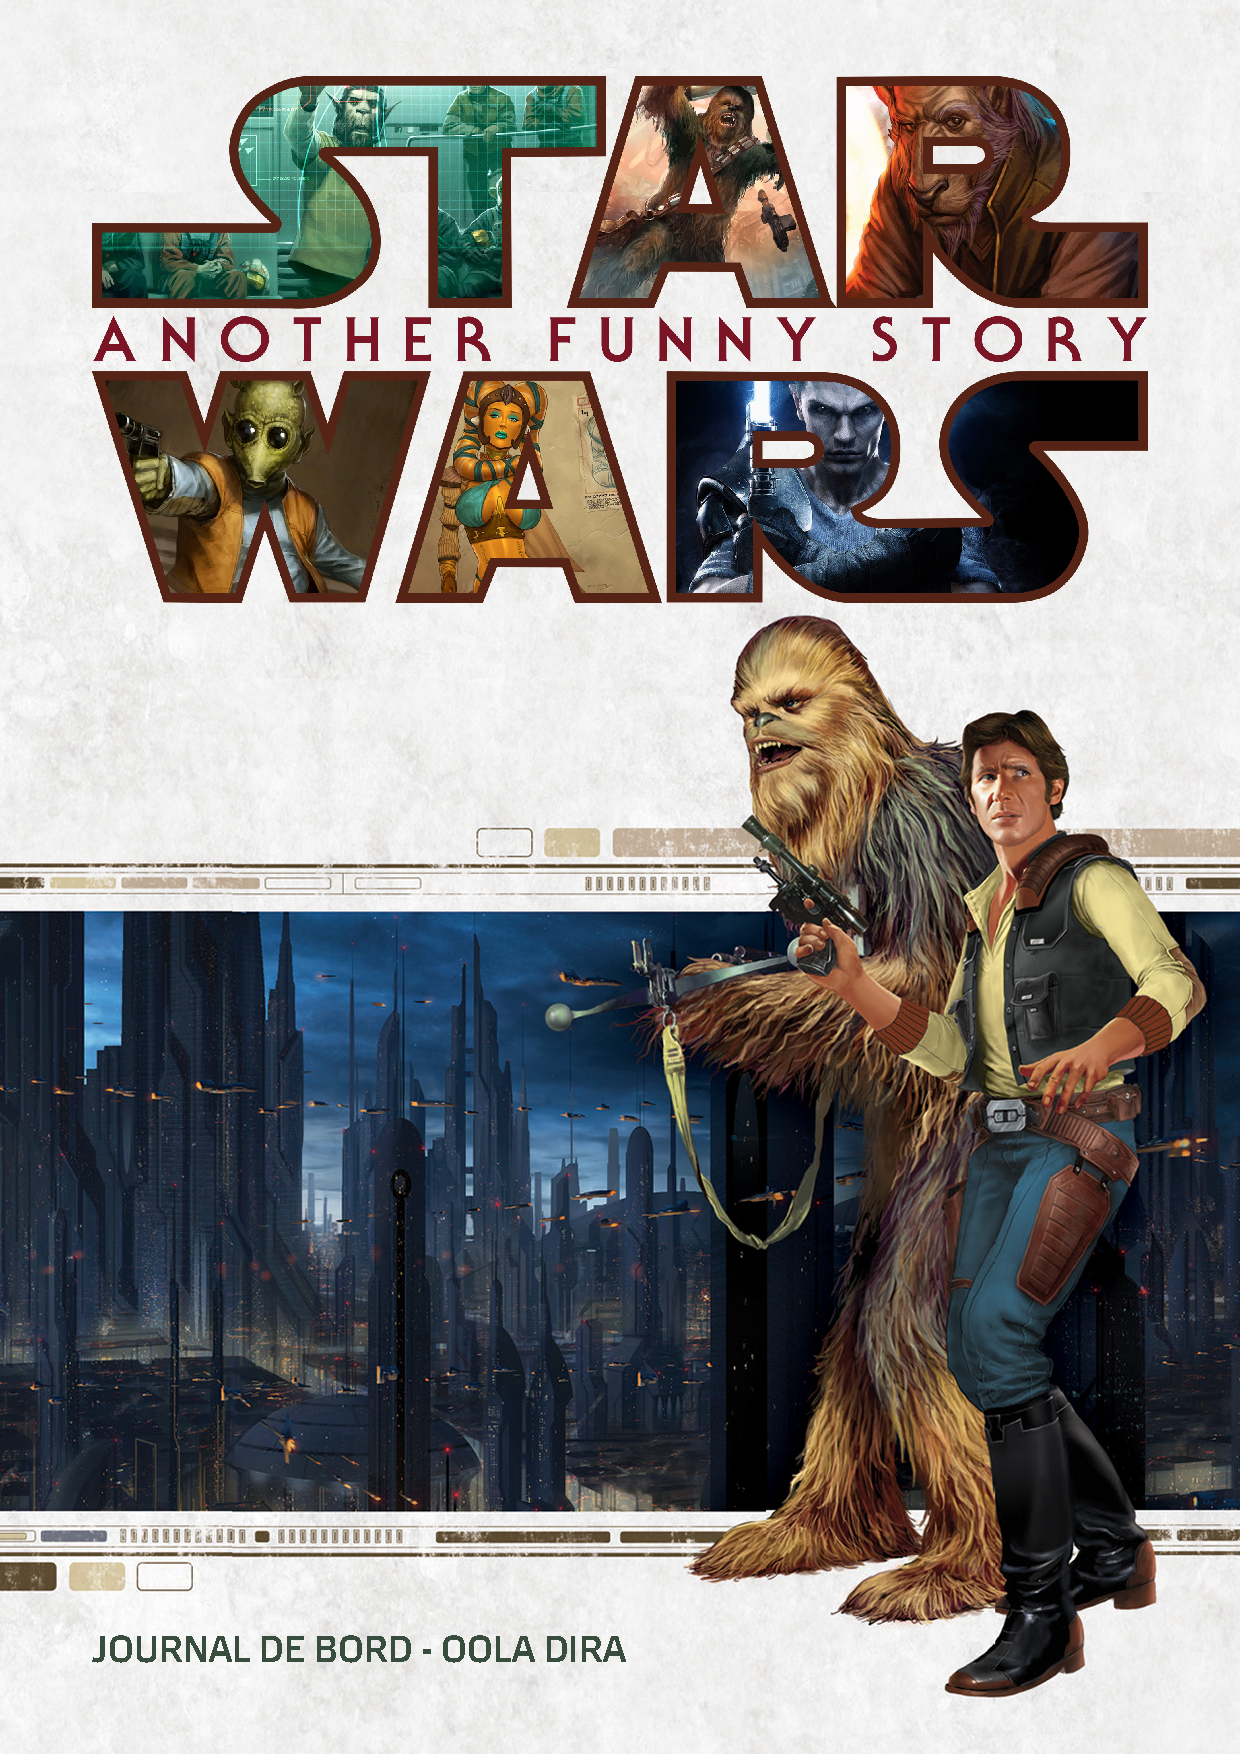
\includepdf[]{img/Front.pdf}

% Seconde de couverture

\chapter{Généralités et Crédits}

\section{Maître du jeu}

\paragraph{Pibeto} Empire, Résistance, Rebelles, Animaux, Ambiance, ... \emph{Merci à lui.}

\section{Joueurs}

\paragraph{`Oola `Dira, (BSJ)} Twi’lek de couleur orange, mécano.
\paragraph{Wesk-Fen Bok 'iort (Fred)} Botan, † dans un combat
\paragraph{Nyr Ch'iort (Natacha)} Botan, signe distinctif des ailes d’anges, pilote.
\paragraph{Wootang (Nboo)} Wookie médecin et éclaireur
\paragraph{Nopok Atol (Ghe)} Rodien verdâtre de 19 ans, chasseur de primes et sniper, † dans un combat.
\paragraph{Kane Starkiller (Rro)} Humain de 23 ans, 1m98, mercenaire maraudeur très bon au corps à corps.
\paragraph{Kar Lya 'Dren (Yo)} Botan, tech/sliceur
\paragraph{Irys Thri 'iya (Christelle)} Botan, disparue à ce jour
\paragraph{Kalcir Thuk} Chasseuse de primes

\section{Le vaisseau}
Cargo léger de type corélien \emph{YT-1300}
\emph{\color{red}\textcyr{ТОВАРИЩ}}

\section{Quelques aides et rappels}

\subsection{Investir}

\begin{dndtable}[p{0.3\columnwidth}X]
  \textbf{Achat}                & \textbf{Description} \\
  Compétence carrière           & 5 * seuil (5, 10, 15, ...) \\
  Compétence hors carrière      & 5 * seuil + 5 (5, 10, 15, ...) \\
  Arbre de spéc.                & 10 xp * nb. tot. specs. \\
  .... si nouvel                & Majoration de 10 xp \\
\end{dndtable}

\section{Symbolique}

\begin{dndtable}[cX]
  \textbf{Dés}                & \textbf{Description} \\
  \boost         & aide, bonus \\
  \setback       & contrainte, malus \\
  \difficulty    & difficulté \\
  \ability       & habilité \\
  \challenge     & challenge \\
  \proficiency   & efficacité \\
\end{dndtable}

\begin{dndtable}[cX]
  \textbf{Symbole}  & \textbf{Description} \\
  \successA & Succès \\
  \failureA & \'Echec \\
  \advantage    & Avantage \\
  \threat       & Menace \\
  \triumph   & Triomphe \\
  \despair   & Fumble \\
\end{dndtable}


\begin{figure}[b]
    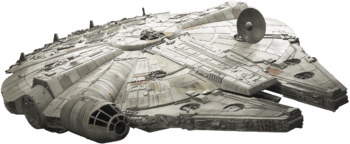
\includegraphics[width=0.45\textwidth]{img/yt1300.png}
    \label{yt1300}
    \caption{\textcyr{ТОВАРИЩ}}.
\end{figure}

\newpage

\tableofcontents

\chapter{Les personnages}

\section{`Oola `Dira}

\paragraph{\^Age} Temps humain … 22 ans
\paragraph{Sexe} Féminin
\paragraph{Race} Twi’lek

\begin{wrapfigure}{O}{0.25\textwidth}
    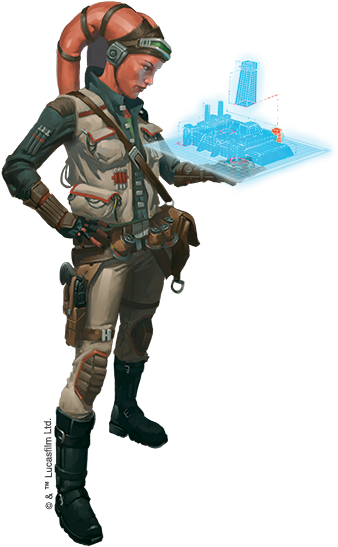
\includegraphics[width=0.25\textwidth]{img/oola.png}
    \caption{`Oola `Dira}
    \label{suskafoo}
\end{wrapfigure}

Oola est née sur Ryloth. Issue d’une famille de marchands son père était spécialisé dans le commerce de Ryll et notamment l’exportation.
C’est ainsi que dans la famille, une tradition de négociations avec les milieux mal famés est née. Afin de gérer au mieux le commerce, son père maîtrisait en particulier le transport afin de mener à bon port ses précieuses cargaisons.
C’est ainsi que très jeune, Oola a appris les bases du commerce, d’astrogation et de mécanique, en accompagnant son père lors de multiples livraisons.

Malgré des affaires florissantes, les activités illégales de son père et ses mauvaises fréquentations lui imposèrent de se trouver une protection à n’importe quel prix. Celui-ci fut terrible puisque ce fut son enfant, Oola. C’est pourquoi à l’âge de 11 ans, Oola a été vendue au célèbre mécanicien Suskafoo (de race Verpine, figure~\ref{suskafoo}) à la capitale de Ryloth : Kala'uun.


\begin{wrapfigure}{I}{0.2\textwidth}
    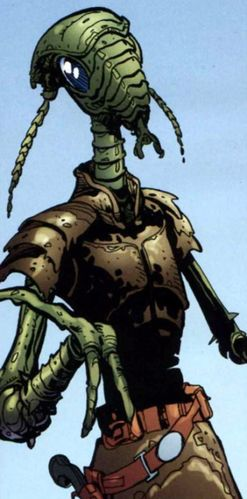
\includegraphics[width=0.2\textwidth]{img/verpine.jpg}
    \caption{Suskafoo}
    \label{suskafoo}
\end{wrapfigure}

Oola continua donc sa vie en esclavage, au service de Kala’uun. En tant qu’esclave elle n’a pas été formée au combat, mais elle a comblé cette lacune par son intelligence qu’elle cultiva par ses rencontres au sein de l’astroport. Elle parvint même à faire sa propre réputation discrète de mécanicienne de génie.

C’est ainsi qu’au fil des ans, Oola réussi a survivre dans ce monde particulier, jonglant entre magouille, bon plans et discrétion, tout en évitant les affrontement, tant que possible. Régulièrement, elle avait à traiter avec un célèbre chasseur de prime Rikta Noor. Les conseils d’Oola sur la préparation de son vaisseau et de son équipement lui sauvèrent la vie à maintes reprises. C’est pourquoi à l’âge de 20 ans, pour la remercier, Rikta racheta Oola.

Durant deux ans, elle le servit avec dévotion et cette expérience lui permet de découvrir de nouveaux mondes. Elle devient une mécanicienne hors pairs.

Deux ans plus tard, le chasseur de prime fut tué au cours d’une mission difficle et Oola en profita pour s’enfuir et se créer une nouvelle vie libre. Cette soif de liberté qui sommeillait depuis des années fit enfin surface et lui donna l’énergie de fuir ces mondes d’esclavage et de misère. Mais ce choix s’accompagne d’une dette qu’Oola se promet de rembourser. En effet, Rikta Noor a eu une fille, qu’il a conservée hors de sa vie de tumulte. Puisque Oola était au service de Rikta, elle se doit d’être au service de sa fille, ou au moins racheter sa liberté auprès d’elle.

Ainsi, Oola se met à explorer les différents mondes afin de trouver une planète de liberté.

Elle trouva alors une troupe de voyageurs avec lesquels elle décide de continuer son voyage. Voulant se mettre plutôt à leur compte pour leurs aventures, le groupe contracte une dette financière pour l’achat du vaisseau avec lequel elle part vers de nouvelles aventures.

\chapter{Un petit service}

\section{Contexte de la mission}

Premières informations concernant votre groupe.

Vous possédez en commun un vaisseau qui est un cargo léger corélien YT-1300 sans aucune modification : vous n’avez encore pas eu le temps de le bidouiller à votre convenance.

\begin{quotebox}
Votre vaisseau ressemble extérieurement au Faucon Millenium, mais ce dernier a été modifié par tous ses propriétaires successifs pour avoir les performances qu’il a dans les films.
\end{quotebox}

C’est un choix intéressant, car il dispose de suffisamment d’espace pour un équipage de 6 personnes, et offre des compartiments de stockage assez vaste pour transporter des marchandises en quantités suffisantes pour faire du commerce (licite ou non). Il ne vous reste plus qu’à lui trouver un petit nom !

\begin{quotebox}
J’attends d’avoir la totalité des fiches de chacun pour vous donner un briefing plus général sur votre situation. Je peux par contre déjà vous dire où vous êtes lors du début de l’aventure)
\end{quotebox}

Un ami proche du groupe, vous a contacté sur Coruscant, pour vous demander de lui rendre un petit service rémunéré. Il souhaitait faire transporter une cargaison d’évaporateurs, de Coruscant vers Tatooine afin de dépanner un oncle opérant une ferme hydroponique. Vous toucherez 3000 Crédits à la réception de la marchandise à Mos Eisley, chez Carl Moody (l’oncle de votre ami)

L’aventure commence pendant le vol en Hyperespace…

\section{Une alarme se déclenche}
\subtitle{ 1\ier{} mai 2014}

Nous avons un vaisseau d’occasion et 3000 crédits pour livrer les évaporateurs. Cette mission classique est estimée à 2 semaines de voyage. Nous découvrons notre vaisseau qui est composé de plusieurs pièces, dont 3 emplacements secrets.

Durant le voyage, une alarme se déclenche...

\section{Une nouvelle mission se présente}
\subtitle{12 octobre 2014}

Sur la planète Corellia et la lune de Dral, Prisoa devient une base arrière. Un évaporateur est à livrer sur Tatooine au plus tôt, le retard n'est pas une option.

Un hutt, que nous ne connaissons sans plus.

\chapter{Objectif : Capture}

\begin{commentbox}{Discussion avec Jeroh Sullustéan}

Un créancier a lancé une chasse à l'homme sur Formos, demande de participer à la chasse contre Dobah de la race des Aqualés. Je tente un jet de charme, mais ce dernier est raté, mais quelques conseils nous sont fournis\ : il faut y aller. On peut le recontacter.
\end{commentbox}

Sur Bandin, nous avons quelques informations complémentaires sur Dobah. C'est un fameux pirate de la passe de Kessel. Il se coltine plusieurs primes, dont une de 10 000 crédits par Moruth Doll ainsi qu'une prime de 5 000 par Bekta Bessoui Dori, mais vivant cette fois-ci.

Nous partons donc en direction de Formos, et le trajet nous prend 8 jours. Afin d’accéder à l'astroport, nous devons débourser 150 crédits.

Afin de récupérer quelques informations, nous nous dirigeons naturellement vers la cantina. Mais sur le chemin, nous remarquons un speedster dont le chauffeur fait le guet, et non loin de là, une bande sort d'un trou avec 3 caisses. Naturellement, nous engageons le combat, et récupérons dans les caisses, des datapads dont nous nous en attribuons un chacun.

\section{Altercations à la cantina}
\subtitle{Journal du Sergent Cody, Corps expéditionnaire de la planète Formos. \newline 9 décembre 2014 }

Des activités criminelles ont été rapportées dans l’après-midi et en début de soirée dans les environs de la Cantina.

3 hommes ont été sauvagement assassinés à l’arme blanche aux abords d’un entrepôt qui venait d’être cambriolé. Un groupe de suspect a été aperçu s’enfuyant des lieux par une patrouille qui a fait les premières constatations.

Un peu plus tard des échanges de tirs ont eu lieu à la Cantina. 2 victimes sont à déplorer. Il s’agit de 2 pirates bien connus de nos services. Les quelques témoins ont fait part d'un groupe d'étrangers correspondant au signalement des tueurs des premiers meurtres.
Un règlement de compte serait-il en train de se passer entre les différents cartels\ ? Une bande de drogués aux Glitterstim serait-elle à l’œuvre\ ? La prime pour Dobah est-elle la cause de ce bain de sang ?

J’ai demandé à renforcer les patrouilles pour que la zone reste calme, mais je crains que les incidents continuent tant que les suspects n’auront pas été appréhendés.

\section{Que l’Empereur veille sur nous !}
\subtitle{14 décembre 2014}

À la cantina R. Rigens, nous apprenons que Daro Blunt serait de mèche avec Dobah. Nous rencontrons une rodienne Zukata qui nous signale que Kessel est vraiment une zone dangereuse et mal fréquentée, bien qu'elle soit chargée d'histoire. De plus nous apprenons qu'elle offre 2000 crédits si nous arrivons à retrouver le droïde R4W9. Le frère de Zukata, Godon Mekata a disparu alors qu'il était à la recherche de Dobah. Pour information, elle loge à l'hôtel Excelsior.

Wesk-Fen voit un toydarien sortir de la cantina et en profite pour le poursuivre jusqu’à un entrepôt où nous la rejoignons.

Trouvant cette activité louche, nous attaquons sans ménagement. Je tente d’user de mon charme pour infiltrer le bâtiment, sans aucun succès et je finis par me faire tabasser. Mais au terme du combat, nous trouvons quelques crédits que nous nous partageons (+50) ainsi que le droïde R4W9. 

Nous le ramenons à Zukata qui nous paie les 2000 crédits.

De retour au vaisseau, nous partons à la vitesse lumière vers nos prochaines aventures, tout en profitant de quelque repos. Malheureusement interrompu par une sortie d'hyperespace tout proche d’un astéroïde que nous avons détecté. Cet astéroïde est un vrai gruyère plein de cavernes. Nous décidons d’atterrir en A et rentrons dans le boyau du vers de l'espace.

Nous y trouvons un premier vaisseau monoplace qui semble en bien mauvais état, complètement Hors-Service. Il appartenait à Godon Nétaka.

Lors de la fouille du vaisseau, StarKiller y trouve :
\begin{itemize}
\item 5 grenades à Hélium (elles permettent de buter les chauves-souris (Minock)
\item 2 bâtons luisants
\item 6 paires de menottes (nous n’en gardons que 5).
\end{itemize}

Nous continuons notre exploration et trouvons dans B, 10 Minock … Et enfin, la caverne C. Nous y découvrons un sas pressurisé contenant 6 personnes. Après avoir déposé Kar et StarKiller, nous tirons et ratons grossièrement. Après le combat, la fouille s'avère fructueuse :
\begin{itemize}
\item 530 crédits
\item 3 carabines blaster
\item 1 paire de gants à décharge (Star killer)
\item 1 gourdin en acier
\item 500 autres crédits de la sentinelle
\item 1 caisse de Glitterstim (x100) pour environ 5000 crédits
\item 50 Glitterstim
\item 4 Pistolets blaster lourd.
\end{itemize}

Nous devons à présent repartir et 3 choix se présentent à nous :
\begin{itemize}
\item La passe de Kessel pour l’empire
\item Sleheyron pour retrouver le Hutt
\item Formos pour y retrouver Zukata
\end{itemize}

Nous retournons donc voir Zukata pour l’informer que nous avons retrouvé le vaisseau de son frère.
Puis nous continuons le voyage vers Sleheyron voir Tabar. En arrivant à l'astroport, je reste au vaisseau. Nous y gagnons\ :
\begin{itemize}
\item 3750 crédits répartis
\item 1 kit de crochetage pour Wesk-Fen et un lance-torpille à proton, monté sur l’appareil, avec 1 torpille.
\end{itemize}

Dobah est aux arènes de la mort et nous gagnons 5000 crédits pour la prime partagée.

\section{Une erreur de jugement}
\subtitle{25 janvier 2015}

Nous avons un prisonnier en soute du nom de Alger Sodert. Afin de tenter de le fouiller et voler son arme, je tente de le droguer. Mais au moment d’ouvrir le sas, je me laisse surprendre et par "réflexe", je l'exécute sans ménagement.

Étant seule dans le vaisseau, je reste désemparé quant à mon action et des conséquences qui doivent en découler, notamment sur la partie nettoyage. Finalement, je rejoins le reste de l'équipage voir Tbakbe pour tenter de négocier un pistolet disrupteur.

Encore une fois, mes tentatives de négociations s’avèrent veines !

Par chance et manque de temps, l’histoire du cadavre dans le sas a été mise de côté.

\chapter{Des Ugnaught en pagaille}
\subtitle{2 avril 2016 \newline Scénario custopn \newline Présents\ : NBOO (Wootang), Nat, Yo (Karka), Rro, Ghe (Nopok), BSJ}

De SléEyrone, j'arrive en navette à l'astroport de Christophsis afin de rejoindre l'équipe qui était partie sur une autre mission. Ils ont trouvé une lettre d'échange pour 200 esclaves (Ugnaught, \ref{ugnaught}) et sont partis pour les récupérer. Pour cela, ils louent à Krall (toydarien), un vaisseau de transport, mais ce dernier les double et part avec le vaisseau. Un désir de vengeance les mène à le poursuivre et à enquêter sur Weksol.

\begin{wrapfigure}{O}{0.25\textwidth}
    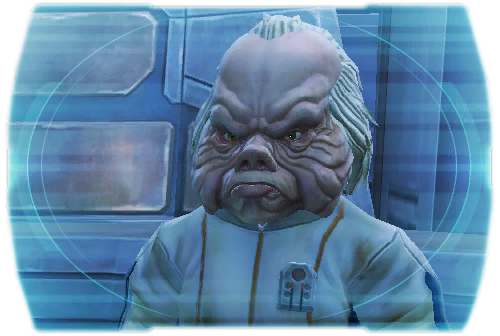
\includegraphics[width=0.25\textwidth]{img/ugnaught.png}
    \caption{Ugnaught}
    \label{ugnaught}
\end{wrapfigure}

Grâce au piratage d’une console avec l'aide de Karka, nous trouvons quelques informations sur le gouverneur Weksol. Il semble être associé au Soleil Noir, un groupuscule de contrebande. On trouve en particulier un listing avec des informations sur les propriétés et les revenus de cet individu qui sont datées jusqu’à ce jour.

Afin d’obtenir des informations complémentaires, nous nous dirigeons à la cantina en laissant Karka en train de hacker l’ordinateur trouvé, et Nopok demande des informations à la guilde des chasseurs de prime. Grâce à ma perception, je remarque que nous sommes suivis, mais je perds de suite la trace de l’individu.

À la cantina, je remarque directement 2 gars qui discutent\ : un wookie et un mon calamari du nom d’Ikaba. Parlant de «\ gâteaux\ », je soupçonne facilement qu'ils parlent de trafic et grâce au SystemD, j’arrive à tirer quelques informations, et notamment un contact du nom de Dootik au Hangar 13 à l'astroport de Christophsis.

Après cette discussion, retour au hangar du vaisseau ou nous retrouvons Nopok qui nous rapporte les informations qu'il veut bien partager. Weksol est donc un représentant de l'empire. La guilde des chasseurs de prime propose en effet tout un tas de primes sur divers trucs, notamment des primes de 1000 crédit sur Ropok et Cratala.

\begin{wrapfigure}{O}{0.25\textwidth}
    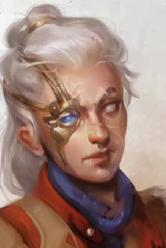
\includegraphics[width=0.25\textwidth]{img/cratala.jpg}
    \caption{Cratala}
\end{wrapfigure}

Karka a finalement réussi à trouver de plus amples informations sur l'ordinateur hacké. En effet, sur un astéroïde proche, il a contacté de nombreuses livraisons pour un soi-disant hôtel en construction depuis plusieurs années.

Au même instant, un étrange individu nous attend à la porte du hangar et nous conseille vivement de nous barrer au plus vite, car l’exécution de notre chauffeur de taxi ne semblait pas nous avoir persuadé que nous n’étions pas vraiment acceptés dans les parages. Après discussions entre nous, nous choisissons de partir vers la roue, mais en faisant tout de même un détour vers l’astéroïde pour voir ce qu’il en est.

En trajet vers l’astéroïde, nous remarquons que nous sommes suivis, arrivés près du soi-disant hôtel, un scan nous permet d’identifier 200 formes de vie, 2 vaisseaux de transport ainsi que des petits vaisseaux.

Contre les recommandations de StarKiller, qui s’ennuie visiblement de ces investigations, nous décidons de nous attaquer à cet hôtel ainsi qu’à nos poursuivants.

Les combats s’engagent mais avec force et bravoure, nous réussissons à délivrer les 200 Ugnaught de leur prison. De retour vers les vaisseaux de transport, nous sommes surpris par quelques forces massives, qui, après avoir étourdi la plupart d’entre nous, sont des "amis" pour ce jour, dont le gouverneur Weksol.

Nous accompagnons donc les Ugnaught vers une planète neutre Excarga à bords de notre vaisseau ainsi que d'un GR75 où ils connaissent une cache des contrebandiers que nous venons de combattre. Cette cache renferme pas mal de matériel :
\begin{itemize}
    \item 10 blasters lourds
    \item 10 blasters légers
    \item 2 pistolets disrupteurs
    \item 1 kit générateur de bouclier
\end{itemize}

Je prends donc 1 des 2 pistolets disrupteur de cet arsenal afin d’améliorer mon équipement qui est tout de même succinct.

Le fait d’avoir aidé les Ugnaught qui sont des mécanos aguerris, nous a permis d’obtenir leurs faveurs (ils se méfient tout de même de moi, car je suis Twi'lek, comme leurs ravisseurs) et nous assurent que nous pourrons compter toujours sur les Ugnaught au travers de la galaxie.

Cette mission m’a permis de me réconcilier avec mon vœu de propager la liberté au sein de la galaxie, c’est pourquoi je gagne 25 XP. Mais il me reste une blessure critique à la tête (50) et un taux de blessure de 9/11. Le vaisseau a été aussi pas mal endommagé.

Nous restons une semaine sur Excarga et pendant cette période de repos, j’en profite pour me soigner critique et normal et réparer le vaisseau à l’aide des Ugnaught et monter le générateur de bouclier. Utilisation de réparation solide (restaurer +1 dégât de coque)

\chapter{Les charlots en mission}
\subtitle{May the 4th, 2016 \newline Scénario custom}

Une semaine sur Excarga, qui m’avantage grâce à son climat aride, me permet de m’entraîner dans mes compétences et notamment sur :
Une ceinture à gadgets
Une compétence de Bidouillage appliquée sur pistolet disrupteur afin de baisser son critique de 1.
Ainsi qu’être inventeur afin de se focaliser sur l’entraînement.

De plus, Wootang me soigne de mon critique moyen (50) et de mes blessures grâce à un succès.

Nous nous ennuyons fermement à présent et traînons pas mal au \emph{Benta Assoiffé} pour passer le temps. En ville, nous trouvons une boutique où une \emph{robe} de Jedi fait de l’œil à StarKiller, mais son prix de 4500 crédits le bloque franchement. Pendant ses tentatives de négociation, j'arrive à trouver pour 150 crédits, un sac à dos modulaire qui me permettra enfin de transporter tout mon matériel de bidouillage.

Après pas mal de discussions, StarKiller arrive à trouver une piste de mission qui nous permettrait de récolter 4000 crédits, que nous répartirions entre nous quatre. En effet, un certain Lidan Kegel, chercherait à partir de la planète. Il attend au \emph{Benta Assoiffé}.

Nous nous rendons donc à la cantina, afin d'essayer de trouver ce Lidan. Pour ma part, je tente, en vain de me lier d’amitié avec \emph{Ilock} le patron du bar, Twi'lek aussi, mais me prenant les pieds dans le tapis comme d’habitude, j'arrive au moins à payer des bières, à savoir qu’un Duro traite des affaires louches et que le patron de la boutique n’est pas de toute confiance.

De son côté, StarKiller trouve Lidan Kegel qui veut aller à Banistar mais a besoin de faire un détour pour récupérer quelques documents. Il ne peut pas utiliser les transports classiques, car il est recherché. Tant et si bien que StarKiller arrive à négocier 6800 crédits son transport, en incluant la génération de faux papiers... loin d’être notre spécialité.

Afin de savoir comment s’en procurer, nous convainquons notre slicer de hacker le site des douanes à partir d’un cybercafé (et non pas de notre vaisseau) afin d'avoir plus de renseignements sur le site de douanes. Il finit par trouver les plans du bâtiment, tout en déclenchant toutes les alarmes informatiques possibles et imaginables. StarKiller et Karka, le Pierre Richard de l'informatique. Nous nous échappons tout en menaçant le jeunot du cybercafé de se la fermer. Deux speedsters du service d’ordre arrivent promptement à l'instant où nous partons. Je tente de rester un peu, afin d’avoir quelques infos, mais StarKiller m’en dissuade et nous partons reconnaître les lieux de la douane, afin de trouver comment obtenir des papiers pour Lidan.

Après avoir repéré les lieux, nous décelons un système de sécurité conséquent, mais aussi un système de ventilation qui peut être accédé à partir du toit. Nous gardons ces éventualités en mémoire et retournons à la cantina afin de tenter d’acheter des papiers directement à un Duro (Illustration~\ref{duro}).

\begin{wrapfigure}{O}{0.25\textwidth}
    
\includegraphics[width=0.25\textwidth]{img/duro.jpg}
    \caption{Duro}
    \label{duro}
\end{wrapfigure}

Ce dernier est en pleine discussion avec un weequay lorsque nous arrivons à la cantina, je tente une approche mais me fait refouler directement. La patience légendaire de StarKiller ne suffit pas à le retenir de tenter sa chance aussi, mais la main sur la garde de son arme. L’intimidation semble fonctionner et le weequay va rejoindre sûrement ses acolytes à l'entrée de la cantina pour nous préparer une belle sortie. Les négociations avec le duro sont difficiles et nous finissons par laisser tomber et choisissons de nous attaquer directement au bâtiment des douanes.

À la sortie de la cantina, nous restons vigilants, mais le weequay ne semble plus être là. Nous allons alors directement au bâtiment des douanes. StarKiller et Wootang montent directement sur le toit, moi-même, n’étant point trop agile, je monte sur le toit du bâtiment adjacent afin d'y trouver une autre voie, mais je n'arrive pas à y accéder. Je choisis donc de faire le guet au pied du bâtiment.

StarKiller et Wootang hissent Karka sur le toit car lui seul semble apte à hacker les terminaux pour générer un droit de sortie en bonne et due forme. Après quelques erreurs d'orientations et quelques boulettes sans conséquences (on est maladroit ou pas), Karka arrive à obtenir une clef de sortie pour Lidan, mais sa présence semble être découverte. Il réussit à s’échapper par la fenêtre en rattrapant la corde tendue par Wootang. Pour finir en toute beauté, Kar glisse en tentant de fermer sa fenêtre de sortie et … choit lamentablement un étage plus bas. Fort heureusement, ce dernier ne meurt pas et me fait une belle frousse, car je pensais que mes acolytes venaient d’être capturés.

Finalement, nous rentrons fissa au FireSpray afin de régler au plus vite cette mission qui est bien mal partie. Après avoir récupéré Lidan, nous partons pour Herdessa afin d’y récupérer des documents exigés par Lidan. Enfin, nous arrivons à faire un truc correctement et parvenons à faire le chemin en 1 journée au lieu de 2.

\section{Une question d’honneur}
\subtitle{28 mai 2016}

Pour rappel, sur Excarga, j’ai pu réparer le vaisseau à l'aide des Ugnaught. En effet, ce dernier était bien endommagé et a nécessité beaucoup de travaux, nous avons dû reprendre la moitié du vaisseau pour le remettre en état. Grâce à mes compétences, il faut l'avouer et l'aide de nos nouveaux amis, on a limité la dépense à 3000 crédits (au lieu des 5500 prévus). Je profite de cet échange avec les Ughnautes pour leur acheter une trousse à outils pour 200 crédits, qui m'aidera bien pour les prochains bricolages.

Pour en revenir à notre aventure, nous accompagnons Lindan vers Herdessa afin qu’il puisse récupérer les documents dont il a besoin. Sur la route, malgré l'inquiétude de Lindan, nous récupérons Nopok et Nyr Ch'iort et laissons Karka et Wootang partir pour la roue avec le FireSpray. Nous continuons donc avec le YT-1300 que nous renommons\ : \emph{\textcyr{ТОВАРИЩ}}.

Nous arrivons donc à Herdessa, planète à 90\% aquatique et atterrissons à Herdessa Prime (200 crédits), étrangement StarKiller adore cette ambiance humide et oppressante de la ville sous-marine que nous découvrons, ambiance qui ne sied guère à Nopok. N'ayant que peu confiance en Lindan, nous l'accompagnons à sa planque pour récupérer les documents et 2\ datapads. Nous remarquons que bien qu'il semble solitaire, il a une famille grâce aux photos visibles à sa planque. Nous ne souhaitons pas nous attarder sur place et retournons au plus vite au vaisseau, mais nous constatons que nous sommes surveillés de près. \emph{Nous …} sauf Nopok, en effet, l'effet de cette ville sous-marine le perturbe pas mal et il ne nous croit pas.

Au moment de décoller, nous sommes poursuivis par un vaisseau qui nous somme de lui livrer Lindan. Après un court échange, très peu courtois, nous engageons le combat contre Vossirl, le chasseur de prime, car nous ne souhaitons pas nous laisser faire quand-même. Connaissant de mieux en mieux notre vaisseau, nous maîtrisons le combat et notamment StarKiller nous apporte son soutien en ingénierie pour réparer le vaisseau et préparer quelques disciplines de Tir pour garder le dessus. Une fois le combat gagné, nous filons sur Station Bannistar afin d’emmener à bon port Lindan, qui s’avère être ingénieur et se propose de m’aider à réparer le vaisseau.

Après l'arrimage à 150 crédits, Nyr Ch'iort remarque sur le pont plusieurs vaisseaux portant la marque du Soleil Noir, et même beaucoup. Tous accompagnent Lindan chez lui pour qu’il puisse nous régler la mission de transport tandis que je reste au spatioport pour réparer le vaisseau suite aux dégâts subis lors du combat. J’arrive à réparer le critique sur les boucliers et trouve les pièces pour la réparation du vaisseau à 1000 crédits. Je constate que nous sommes encore surveillés par un technicien qui manipule la même caisse depuis plus d’une heure.

De retour au vaisseau, Nopok nous fait un compte rendu de ses investigations au sein de la guilde des chasseurs de prime. En effet, Vossirl était bien un chasseur de prime de sa propre guilde qui était à la recherche de Lindan. Ce dernier était recherché par l’empire. Il nous parle aussi de Bella, une chasseuse de prime réputée et qui rôde dans le coin. De plus, Lindan a retrouvé sa famille sur Station Bannistar.

De son côté, StarKiller tente de surveiller en vain le technicien qui nous observait (tu m’étonnes\ ! Avec l’arsenal qu’il porte, il a du mal à se faire passer pour un mécano). Et c’est à ce moment qu’une belle femme, armée jusqu’aux dents (ce qui semble plaire à certains), s’approche de nous et engage la discussion.

C’est Bella qui vient nous proposer de travailler pour le Soleil Noir si nous lui livrons Lindan. Bien que nous l’ayons déjà déposé, elle nous laisse 30 minutes pour faire notre choix et le lui livrer. Nous discutons âprement sur le fait de lui livrer un père de famille, se mettre à dos ou non le Soleil Noir, garder notre liberté ou tenter de négocier. Finalement, nous choisissons de garder notre indépendance et filons sur Excarga afin d’acheter la robe renforcée tant voulue par StarKiller. C’est en arrivant là-bas, que StarKiller y croise son idole Boba Fett, à qui nous mentons clairement sur l'endroit où nous avons laissé Lindan. Bien nous en a pris d'éviter le conflit pour une fois. Arrivés sur Excarga, StarKiller fonce chercher sa tunique et me laisse son armure matelassée.

Nous restons tout de même un peu sur la planète afin de réparer (encore) le vaisseau et c’est à ce moment que l’on repère le Jump Master de Krall que nous avions identifié sur Christophsis. Par un désir de vengeance, nous choisissons de le retrouver afin de régler nos comptes avec lui.
On repère ainsi le toydarien et 4 de ses acolytes au hangar de leur vaisseau. Nopok se place en sniper au sommet du bâtiment voisin et le reste de l'équipe au rez-de-chaussée pour mener le combat. Nopok met à terre Krall et le combat s'engage au sol. Assez rapidement, nous réglons cette affaire et je constate l'efficacité de ma nouvelle arme\ : \emph{le disrupteur}. Bien qu’illégale, cette arme est sacrément efficace.

Ce remue-ménage attire la bande locale avec laquelle nous avons déjà eu quelques démêlés au \emph{Benta Assoiffé} et enchaînons le combat. Rondement mené, Nyr Ch'iort souffre quand même de quelques blessures et supposant l’arrivée des renforts de la bande de motards, nous choisissons de nous replier au plus vite au vaisseau afin de nous diriger vers «\ la roue\ » où nous attend le reste de l’équipe.

\chapter{À la recherche du vaisseau perdu}

\section{La roue}
\subtitle{10 juin 2016}

On repart à la roue. Chemin faisant, nous rencontrons un chasseur de prime qui prévient Nopok qu’il a une prime sur lui, ainsi que sur la plupart des membres de notre équipe. De plus, afin de trouver une nouvelle mission, Nopok a eu quelques informations sur un Twi'lek du nom de Réom qui pourrait nous embaucher.

Nous nous retrouvons avec 2 vaisseaux, ce qui coûte très cher et choisissons de retourner sur Christophsis pour le vendre. Nous rencontrons alors Boc au hangar 27b. Ce Duros est dur en affaires et finalement, nous arrivons à vendre notre FireSpray pour 10\ 000 crédits.
Nous allons donc sur la roue qui est connue pour ses casinos et ses hôtels. Suite à l’assassinat du sénateur par un groupe rebelle, aucun dirigeant n’a repris le flambeau c’est ainsi que la Roue est sous un régime neutre et autonome. L’empire y est donc officiellement absent.

Pour 1000 crédits nous y atterrissons et j’entreprends les réparations du vaisseau Tovarish (3 heures, 1500 crédits).

Le reste de l’équipe va donc d’une part faire quelques emplettes et d’autre part va à la rencontre de Reom. Ce dernier est PDG d’IsoTech, une société de vente et d’achat de matériel informatique. Il renseigne Nopok sur une mission\ : retrouver le Sa Nalor.

Ce vaisseau a disparu à proximité de Cholgana qui est une planète tropicale recouverte de jungle. C’est un milieu hostile peuplé d’animaux dangereux. La prime est sur une base de 10\ 000 crédits qui pourraient être triplée si la technologie présente est intéressante.

Afin de nous guider et nous épauler dans cette mission, Reom nous confie un droïde ayant quelques informations complémentaires sur la mission. Malheureusement, ce dernier se fait kidnapper par le clan de Yiyar nous supposons, car ce dernier est activement à la recherche du vaisseau. Nous réussissons, au prix d’une course poursuite à récupérer le droïde de leurs mains, mais nous créons pas mal de grabuge au sein de la ville.

\section{Découverte de Cholgana}
\subtitle{30 juillet 2016}

Nous arrivons au hangar et choisissons de repartir au plus vite de la planète quitte à négliger les procédures de décollage, aussi bien administratives que de sécurité. C’est comme cela que nous nous retrouvons nez à nez avec un vaisseau cargo que Nyr évite de justesse. Finalement, nous partons vers les dernières coordonnées connues de Cholgana.

Chemin faisant, je retire le bouchon d’entrave du droïde qui nous apprend qu’il se nomme IT3PO et est au service de Reom. C’est un de ses conseillers financier et technique qui a appartenu au père de Réom\ : Ropok. Il connaissait l'accord commercial qui existait entre Ropok et Harsol sur le partage de découvertes en cybernétique.

Finalement, nous approchons de Cholgana. Cette planète est vaste et les capteurs ne détectent pas grand-chose. Après quelques réglages de capteurs, nous trouvons deux sites sur l’hémisphère nord.

Site 2\ :

Nous retrouvons une capsule de survie 34BH. Celle-ci semble avoir été attaquée par des Nexu, et la boîte noire révèle quelques informations. Notamment que Cratala menait une révolte contre le sénateur.

Suite au combat contre des pieuvres arboricoles, nous repartons dormir en orbite pour visiter le site 1 le lendemain.

Site 1\ :

Nous allons vers le site voir la portion du vaisseau composée de moteur qui a créé un barrage naturel sur la rivière. Nous constatons quelques traces de vie récente comme une barque qui n’a pas plus de quelques mois. Depuis le barrage, nous apercevons plus au nord une forêt étrange qui s’avère être peu naturelle. En effet, lorsque nous nous y rendons et stationnons au-dessus, nous remarquons que la végétation qui y pousse a été mise en place pour camoufler le restant du vaisseau.

Nous nous y faufilons afin d’explorer le vaisseau. Nous avançons avec méfiance, car nous y avons détecté plusieurs traces de vie.

\section{Les féroces nexus}
\subtitle{01 octobre 2016}

Une fois entré dans le cockpit, nous choisissons de continuer notre exploration. Et afin de rentrer dans les tréfonds du vaisseau obscur, StarKiller récupère auprès de Kar sa lampe à fusion pour être notre éclaireur. De mon côté, je bricole un câble afin de pouvoir nous aider dans la descente au travers du vaisseau. De son côté, Kar Lya 'Dren confirme la forme de vie que nous avons détectée. StarKiller descend. De mon côté, je me casse encore la gueule en descendant. Dans l’obscurité des couloirs, la peur se fait sentir et nous dégainons nos armes afin de nous encourager à pénétrer dans ces boyaux obscurs.

Le vaisseau est globalement détruit et en mauvais état, mais nous apercevons un couloir plus dégagé sur notre droite et débouchons sur une grande pièce. J’y détecte un puits en son centre et suivons les signes de vie dans la pièce. Dans un coin obscur, un semblant de tronc est présent et grouillant. Nous y reconnaissons des rats d’écorce. Ce sont des animaux avec un fort instinct de meute, nous choisissons de ne pas les attaquer. On continue alors notre exploration dans un couloir adjacent, tout en marquant notre passage. On trouve une salle plus petite, qui semble avoir été fouillée de fond en comble, mais Nyr y trouve un fusil caché. Pour ma part, je me rappelle avoir au fond d’une de mes poches, une petite lampe. La pièce étant un cul de sac, nous retournons sur nos pas, c’est là que Kar Lya 'Dren nous interpelle au comlink …

\begin{wrapfigure}{O}{0.25\textwidth}
    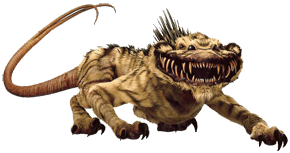
\includegraphics[width=0.25\textwidth]{img/nexu.png}
    \caption{Nexu}
\end{wrapfigure}

Un Nexu nous tombe dessus, rapidement accompagné de deux de ses acolytes. Ils semblent étranges et surtout leurs dents métalliques nous annoncent quelques soucis. Très rapidement, je tombe de mes blessures, en me faisant surprendre par leurs bonds. Nyr est aussi blessée gravement, mais c’est StarKiller qui s’est légèrement trompé de cible.

Le reste de l’équipe arrive à contrôler les animaux qui s’enfuient au travers des couloirs. Après avoir été soignés par Wootang, nous tentons de les poursuivre afin de finir le combat.

Nous les voyons s’enfuir dans une ouverture au plafond, mais les tirs de Nopok ont affaibli le vaisseau et le sol se dérobe sous les pieds StarKiller et de Wootang. Ce vacarme dérange des rats d’écorce que nous exterminons assez rapidement. Nous remontons à la poursuite des Nexus et Kar Lya 'Dren nous rejoint.

Grâce au matériel d’escalade, nous montons tous dans le nid des Nexus et affrontons les deux Nexus blessés. Nous gardons en trophée leur queue modifiée de lames acérées. Nous remarquons dans le nid du matériel ancien de plusieurs dizaines d’années mais aussi du plus récent. Nous divergeons vers sur l’origine de ces Nexus\ : fabrication locale\ ? Animaux de labo de l’époque du crash\ ?

Nous nous concentrons sur notre mission, trouver les plans des implants cybernétiques ainsi que du matériel. Ils devraient se trouver plus bas dans le vaisseau, au niveau de soutes\ ? Nous nous rappelons avoir vu quelques ouvertures au niveau de la plage et choisissons de ressortir du vaisseau afin de se reposer et attaquer le vaisseau par un autre voie.

Chemin faisant, les rats d’écorce ne pouvant apparemment plus nous tolérer sur leur territoire, nous attaquent. Il est vraiment temps de sortir afin de se reposer. Même Wootang, notre médecin semble fatigué.

Arrivés au vaisseau, nous redescendons sur la plage pour nous reposer et reprendre le lendemain notre exploration. Après une nuit agitée pour certains, nous détectons l’approche d’un vaisseau dont la signature semble être celle d’un vaisseau de la flotte du clan Yiyar. Nous choisissons de couper notre matériel électronique afin de ne pas révéler notre présence. Et sortons visiter le vaisseau.

Les entrées détectées sont en fait les stations d’arrimage des pods de secours. C’est un lieu de passage et nous pénétrons une nouvelle fois dans le vaisseau. Après quelques culs de sac, on se retrouve encore une fois face à un puits. Nous discutons de nos options afin de continuer notre aventure: continuer d’explorer, aller chercher le treuil dans le vaisseau, se cacher dans la forêt pour attendre l’arrivée du vaisseau inconnu, décoller pour leur mettre la misère… Finalement, le choix est vite fait quand nous sortons, car nous tombons nez à nez avec un genre de diplodocus\ : des Revos.

Ces animaux sont montés par des droïdes de combat de type B1, un homme âgé et un aqualé. C’est à ce moment que IT3PO interpelle l’homme et le nomme Harsol … Il n’est donc pas mort avec le crash. Harsol reconnaît aussi IT3PO et au bénéfice du doute, nous accueille et nous amène à son village. Je prends place au côté de l’aqualé peu bavard et le reste de l’équipe remonte la rivière vers le campement de l’équipage naufragé.

À notre arrivée, ce ne sont pas des cris de joie qui accueillent, mais plutôt une trentaine de rescapés en haillons qui semblent assez remontés contre Harsol. Il semble tenir son village d’une main de fer. Cette situation est difficile à évaluer, en effet, cela fait plus de 20 ans que ce \emph{village} survit au sein de cette planète inhospitalière.

Harsol nous convie à la salle commune où nous rencontrons Cratala la cybernéticienne. Cheveux blancs et yeux laiteux, elle semble tenir une position importante au sein de cette petite société. Nous discutons avec eux très honnêtement. Il nous présente rapidement la situation du camp, et le fait qu’ils sont restés cachés de l’empire et nous demandent s’ils sont encore recherchés. En effet, une prime court toujours sur leur tête, mais nous leur signalons que nous même sommes mis à prix. De plus, nous leur présentons en toute franchise notre mission de mercenaire, payée par Réom (fils de Ropok)\ : trouver les plans cybernétiques et en bonus, nous pouvons garder tout ce que l’on trouve. Nous signalons de même l’arrivée du vaisseau Yiyar.

Nous rendons à Cratala les queues de Nexu récupérées, car ce sont ses créations. Je montre un vif intérêt pour ses travaux.

Après cette brève réunion publique, Harsol nous guide vers nos quartiers et nous quitte afin de faire le point avec IT3PO. Il reste toute même très méfiant, malgré notre franchise. Nous ne savons pas trop ce que donnera la suite des discussions, mais nous restons dans l’optique de garder notre ligne de discussion sur l’honnêteté.

\section{Sauvetage en concurrence}
\subtitle{27 novembre 2016}
Nous restons méfiants envers ce village. En effet, nous avons pu entendre au détour d’une conversation, certaines personnes se demander pourquoi le capitaine nous avait ramenés vivant.
La nuit plutôt agitée nous a tout de même permis de faire le point, notamment sur les objectifs initiaux de notre mission\ :

\begin{enumerate}
\item Trouver Cratala et ses recherches
\item Les recherches de Cratala
\item Des exemples de ses réalisations
\item Un ou plusieurs membres d’équipage
\item Le capitaine Harsol
\item Les coordonnées de l’épave
\item Des éléments du vaisseau
\end{enumerate}

Durant nos tours de garde, Nyr et Karka ont remarqués, au milieu de la nuit, l’arrivée de 5 nouveaux pensionnaires escortés par des gens du village. Cette équipe composée de 3 rodiens et 2 trandoshans nous semble connue, et sont hébergés à côté de notre baraquement pour la nuit.

De son côté, Wootang a passé aussi une nuit pas mal agitée, il a rêvé notamment d’un vaisseau en flamme et d’une femme ayant retenu par la force, un panneau en métal, afin de sauver un équipage. Est-ce un rêve, une vision\ ! Même lui hésite.

De mon côté, je scrute un peu le village et constate les pièces d’artillerie à l’entrée du village. Ces pièces sont très demandeuses en énergie et en gaz, et il semblerait que le stock soit vide! Du coup, pas sûr que leurs blasters soient vraiment chargés, il me semble qu’ils ne les gardent que pour le côté intimidant. De même, le bourdonnement du générateur de secours n’indique rien de bon. La base semble arriver à bout de souffle.

Pendant que l’on prend notre petit déjeuner, nous voyons en effet que le baraquement à côté est bien habité par les nouveaux arrivants, ils ne nous reconnaissent pas bien que nous les ayons déjà croisés. En effet, StarKiller reconnaît l’équipe qui avait enlevé IT3PO.

Sur ce, Cratala nous rejoint pour discuter et nous fait visiter la base.

Le générateur\ : il me paraît à bout de souffle et FenoGamok me le confirme.\ Nous lui proposons des pièces de notre vaisseau, que nous irons chercher plus tard. Je tente d’en savoir un peu plus sur leurs réserves d’énergie, mais Cratala reste très évasive.

L’infirmerie\ : nous y rencontrons Sarena. Elle a été très gravement blessée durant le crash du vaisseau, mais c’est bien une Jedi. Elle se rapproche très vite de Wootang, elle semble en confiance à ses côtés. StarKiller quant à lui est très intéressé par elle et lui montre la poignée d’un sabre laser. Machinalement, elle le récupère par la Force … mais de suite, n’y fait plus attention. Sur ce, Wootang et Star choisissent de rester à l’infirmerie, pour proposer leur aide, auprès de Sarena.

Cage à nexus, réserve d’armes\ : nous finissons notre tour de visite sur quelques bâtiments dont la réserve qui semble plutôt bien gardée.

Je continue mon périple afin de prévenir nos camarades à l’infirmerie que la visite est finie, et chemin faisant, je repère le groupe d’Yyar. Nopok, de son côté, fouille leur baraque sans réel succès.

Harsol veut confronter ces deux équipes qui viennent en même temps les sauver… Le clan de Yyar est représenté par son second, Yav. Il argue qu’il vient en mission de sauvetage. De notre côté, nous essayons de le convaincre que leur but est uniquement la piraterie, mais Harsol reste très méfiant sur la situation et repousse sa décision à plus tard.

Durant le déjeuner, les relations restent tendues, et pour montrer bonne figure, nous essayons de nous rapprocher des habitants. Je vais manger avec FenoGamok tandis que Star et Wootang vont avec l’équipe de l’infirmerie.

Durant l’après-midi, je pars escorté de FenoGamok et quelques droïdes au vaisseau afin d’y récupérer quelques pièces. De son côté Nopok propose son aide pour un tour de garde sur une tourelle de surveillance.

C’est à ce moment qu’il aperçoit, sur le toit du bâtiment central, Yav qui tente de s’infiltrer. Sans hésitations, il tire et le voit disparaître. Toute cette agitation inquiète Harsol, qui n’a pas remarqué Yav. Il doute même du rapport de Nopok.

Mais finalement, Harsol se fait attaquer dans ses propres appartements et le reste du clan sort des baraquements. Le combat fait donc rage à l’intérieur mais aussi à l’extérieur\ ! Grâce à l’équipe présente, et aux tirs précis de Nopok, le clan est vite réduit au silence.

De mon côté, bien que vexée du manque de confiance de nos hôtes, j’arrive sur le vaisseau pour y récupérer des pièces, et constate un autre vaisseau ayant deux formes de vie à l’intérieur. Mais il décolle aussitôt et disparaît à l’horizon. L’équipage, suite à une ultime communication de Yav, a choisi de prendre la fuite. Nous retournons donc directement au camp de base pour faire le point sur la situation.

\section{Une extraction difficile}
\subtitle{8 janvier 2017}

Après le combat avec le clan de Yar, la tension est importante dans le village. Harsol a réussi à capturer le chef de clan encore survivant, mais le \emph{procès} aura lieu le lendemain.

Le matin n’est pas habituel, Karka, lors de son tour de village matinal, remarque beaucoup de mouvements vers la hutte principale et beaucoup d’hommes en armes, dont deux gardes devant le QG. Nous y allons et assistons au discours de Harsol.

Deux points sont mis en avant :
Il faut se débarrasser de Yav
Notre groupe doit être désarmé…

Cette dernière résolution fait beaucoup de tumulte parmi notre groupe, mais aussi auprès des villageois, qui nous faisaient plutôt confiance. Nos négociations ne les convainquent pas. C’est à ce moment que StarKiller remarque le grondement de moteurs et en fait part à Harsol. Nous sortons précipitamment et Nat remarque un SkyWatcher Impérial, accompagné du bruit d’autres véhicules.

L’alarme du village résonne et tout le monde se prépare au combat, et des droïdes sonde descendent de la canopée. À ce moment, tout s’accélère. Wootang et StarKiller sortent du QG vers l’infirmerie et m’indiquant de surveiller Yav, ce que je fais de suite. Ils vont tenter de convaincre Cratala de nous accompagner dans notre fuite.

Yav est encadré par des gardes qui sont un peu perdus par toute cette agitation. Je remarque Yav en train de tenter de se libérer. Je préviens les gardes qui s’écartent un peu de lui. Nopok en profite pour lui tirer dessus. Bien affaibli, il se protège derrière un garde qui finit par l’assommer. J’en profite alors pour l’attacher plus solidement à un poteau. Nopok sort et c’est à ce moment que Karka entre en même temps que Harsol. Ce dernier est très troublé par ces évènements et nous en tient responsable. Il ne nous fait plus confiance. Je tente de le raisonner, de l’assommer mais rien n’y fait. Mais heureusement, finalement je trouve les bons arguments pour le convaincre qu’à ce moment, nous ne sommes pas la menace mais que c’est l’empire.

Au même moment, Nyr s’occupe des droïdes sondes en face du QG. Elle leur tient tête malgré les coups reçus. Nopok va donc l’épauler et arrive à les mettre en déroute.

Le chef de l’empire présent sur place appel à un cessez-le-feu. Les droïdes battent en retraite et Harsol monte sur une tourelle pour négocier. Nous avons jusqu’au lendemain pour nous rendre.

Durant la nuit, nous élaborons un plan d’extraction, et grâce aux Nexus modifiés de Cratala, nous réussissons à sortir du village et rejoindre le vaisseau. La sortie n’a pas été aussi discrète que nous l’espérions, mais nous avons pu éliminer les patrouilles rencontrées et finalement nous atteignons notre vaisseau à l’aide des animaux marins.

Grâce aux talents de pilotage de Nyr, nous nous échappons de la planète en direction de \emph{Raxus Prime}. Cette planète toxique, sous la coupe de l’empire est aussi une base d’échange pour Reom. Les codes d’accès nous permettent de nous rapprocher de la planète, mais une demande d’inspection nous surprend. Nous plongeons alors dans les canyons d’ordures toxiques de la planète. Après une course effrénée, nous arrivons à supprimer nos poursuivants et accédons à la base de Reom.

Reom devrait arriver dans trois jours.

\section{Extrait du journal du professeur Cratala - Raxus Prime}
\subtitle{8 septembre 2017}

\emph{22 ans…}

Cela fait 22 ans aujourd'hui que le crash a eu lieu sur Cholgana. 

Chaque année j’ai une pensée pour tous ceux qui périrent ce jour-là. Toutes ces personnes croisées dans les coursives du vaisseau durant notre fuite devant les forces impériales. Tous ces amis rencontrés lors des différents voyages effectués avec le capitaine Harsol et dont la vie s’est éteinte ce jour-là. Tous ces anciens patients que j’avais guéris. Tous ces cris. Toutes ces vies brisées. 

J’ai toujours pensé que si j’avais été épargnée ce jour-là et les années suivantes, c’était pour que je puisse aider les autres à survivre, pour que je puisse exercer mon art afin de nous aider à quitter cette planète peuplée de dangers mortels.

Au fil des années, j’ai réalisé que le principal moteur de mon instinct de survie avait été la peur. Une peur sourde mais toujours présente. Non, ce n’est pas la peur de la mort qui me hantait : c’était celle d’être retrouvée par l’Empereur ! Je ne voulais pas tomber dans les griffes de cet homme. Je ne voulais pas que mes réalisations puissent lui servir à dominer la galaxie. Je ne voulais plus me retrouver en face de ce monstre…

Après toutes ces années à avoir vécu avec ce poids, je sens enfin qu’il diminue, qu’il s’estompe. 

Petit à petit.

L’équipe que Reom a envoyée sur Cholgana pour nous chercher nous a enfin fait quitter cette maudite planète et j’entrevois maintenant une faible chance de profiter d’une vie plus paisible …. Même si le décor actuel n’est pas encore l’endroit rêvé…. Raxus Prime. La poubelle d’une bonne partie de la galaxie. Lieu de vie des pillards de décharges. Paradis des Jawas….

La rencontre avec cette équipe a été assez mouvementée mais j’ai toujours senti que nous pouvions leur faire confiance. Ils nous ont d’ailleurs protégés durant l’incursion du clan Yiyar et l’assaut des éclaireurs impériaux. C’est aussi grâce à eux, et à mes chers Nexus, que nous avons pu fuir de nuit notre campement pour rejoindre leur vaisseau. La maîtrise de leurs pilotes et de leurs artilleurs a été remarquable lorsqu’il a fallu semer les chasseurs TIE dans les canyons d’immondices séculaires. Même Harsol en a été impressionné.

Heureusement, nous ne resterons pas longtemps sur cette planète fétide, Reom devant venir nous chercher d’ici deux jours. Ici, au moins, nous sommes à l’abri. Loin de ce maudit clan Yiyar et des forces impériales lancées à nos trousses.

Je vais en profiter pour parfaire mon art et essayer de combler le retard de connaissance que j’ai accumulé en ces 22 longues années…

\emph{22 ans…}

\section{Une affaire juteuse}
\subtitle{30 septembre 2017}

C’est au \emph{courrier brisé} que nous logeons actuellement pour attendre Réom et le paiement de la mission. Malgré une apparence de tas de détritus, la base secrète semble par endroits très bien équipée.

Nous devons nous entretenir avec Norta, un Rodien à l’œil cybernétique. En attendant, nous nous dirigeons à la niche du Benta afin de collecter quelques informations. Il s’avère que Norta gère toute la base et ses activités plus ou moins légales. Finalement, nous le rejoignons pour nous entretenir de la suite des évènements.

\begin{figure*}
\centering
    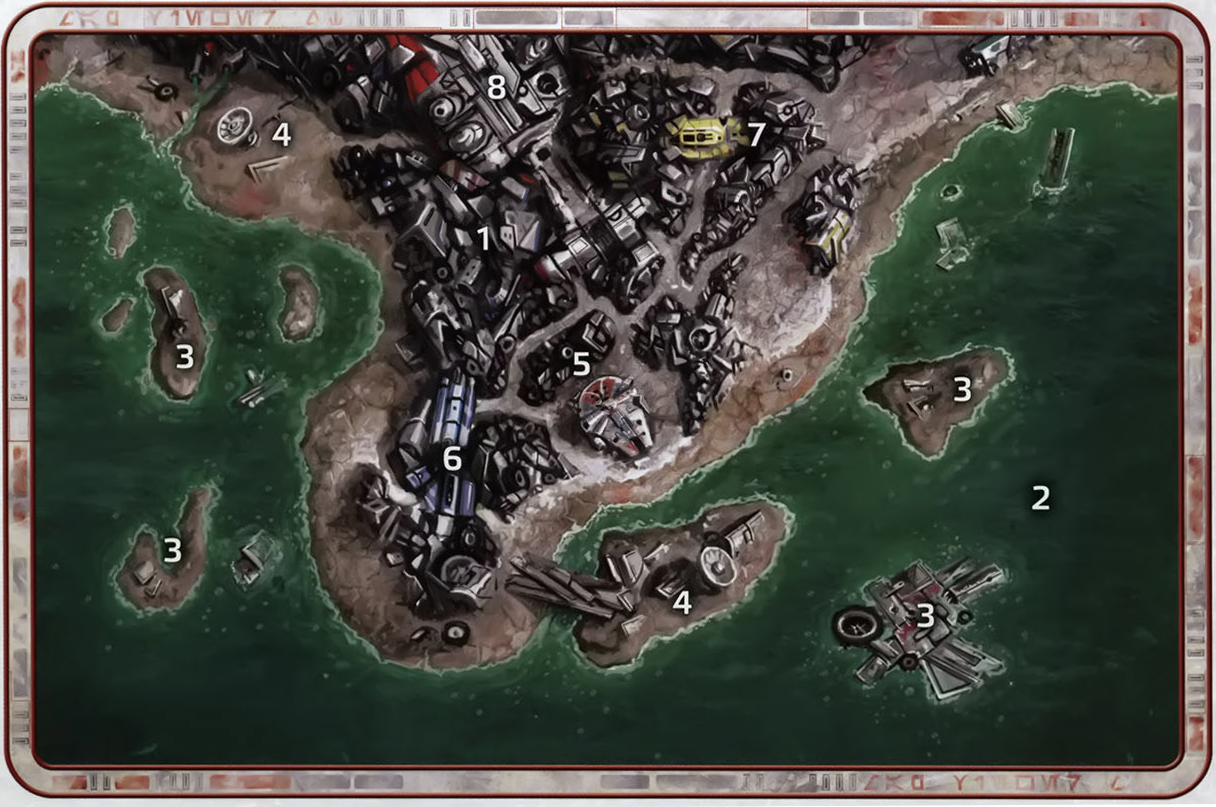
\includegraphics[width=0.80\textwidth]{img/rebut.png}
    \caption{rebut}
\end{figure*}

Cratala, Arsol, IT3PO, Norta nous attendent pour le débrief. En acompte des 30\ 000 crédits attendus, nous en touchons 2000, qui nous permettront de faire quelques emplettes sur la base. De plus, il nous liste quelques raids à faire pour récupérer du matériel. C’est ainsi que nous touchons 14000 crédits pour avoir récupéré un transformateur multiphase et quelques bricoles. C’est en chemin que nous avons rencontré quelques jawa avec qui j’ai pu négocier une caisse de matériel pour construire un droïde contre mon blaster et mon disrupteur. Dans la précipitation de la négociation, écourtée par l’arrivée probable d’une sonde ou d’un tie, les Jawas ont laissés dans la caisse de matériel, un blaster lourd pour droïde. J’en profite d’être sur la base pour racheter un disrupteur pour 3400 crédits.

A notre retour, StarKiller n’est toujours pas rentré de son expédition solitaire, et ne pouvant ressortir durant la nuit, nous patientons au petit matin pour lever une équipe de secours.

Norta nous a indiqué la direction, et nous scrutons attentivement sur le trajet si nous le retrouvons. Finalement, nous lui tombons dessus. Il semble particulièrement affaibli par des combats engagés. Et sur un “malentendu”, il endort Kar. Nous continuons notre mission de sauvetage pour récupérer les corps des camarades de notre pilote qui ont succombés lors de l’altercation avec une sonde. Suite à cela, nous retournons à la base.

Durant notre temps libre, Kar retourne au QG de la base et tente de pirater les ordinateurs de la station. Malheureusement, il se fait attraper et expulser du bâtiment. Ils commencent peut être à se méfier de nous.

Norta nous demande de le rejoindre pour inspecter une livraison de matériel de Jawas. Ce groupe a un comportement suspect et il s’avère que ce sont un Sullustéan et des Trandoshans qui se sont infiltrés ici.

Le combat s’engage et nous entendons qu’il fait tout autant rage à l’extérieur du bâtiment. Nous arrivons à contenir leurs troupes puis à nous échapper pour finalement tomber sur un groupe qui tente d’enlever Cratala.

C’est finalement le clan Yiyar qui est revenu à l’attaque. Grâce aux troupes de Reom qui étaient cachées dans le QG (ce que Kar avait découvert), le clan est vite décimé. Mais tous ces combats ont alertés les troupes de l’empire qui attaquent la base. Nous n’avons que quelques minutes pour nous enfuir. Nous apprenons que le QG est un vaisseau de transport qui peut nous aider à fuir au prix de quelques réparations d’urgence. 

Au prix de quelques dizaines de minutes, nous arrivons à faire décoller le vaisseau.

\begin{figure*}
\centering
    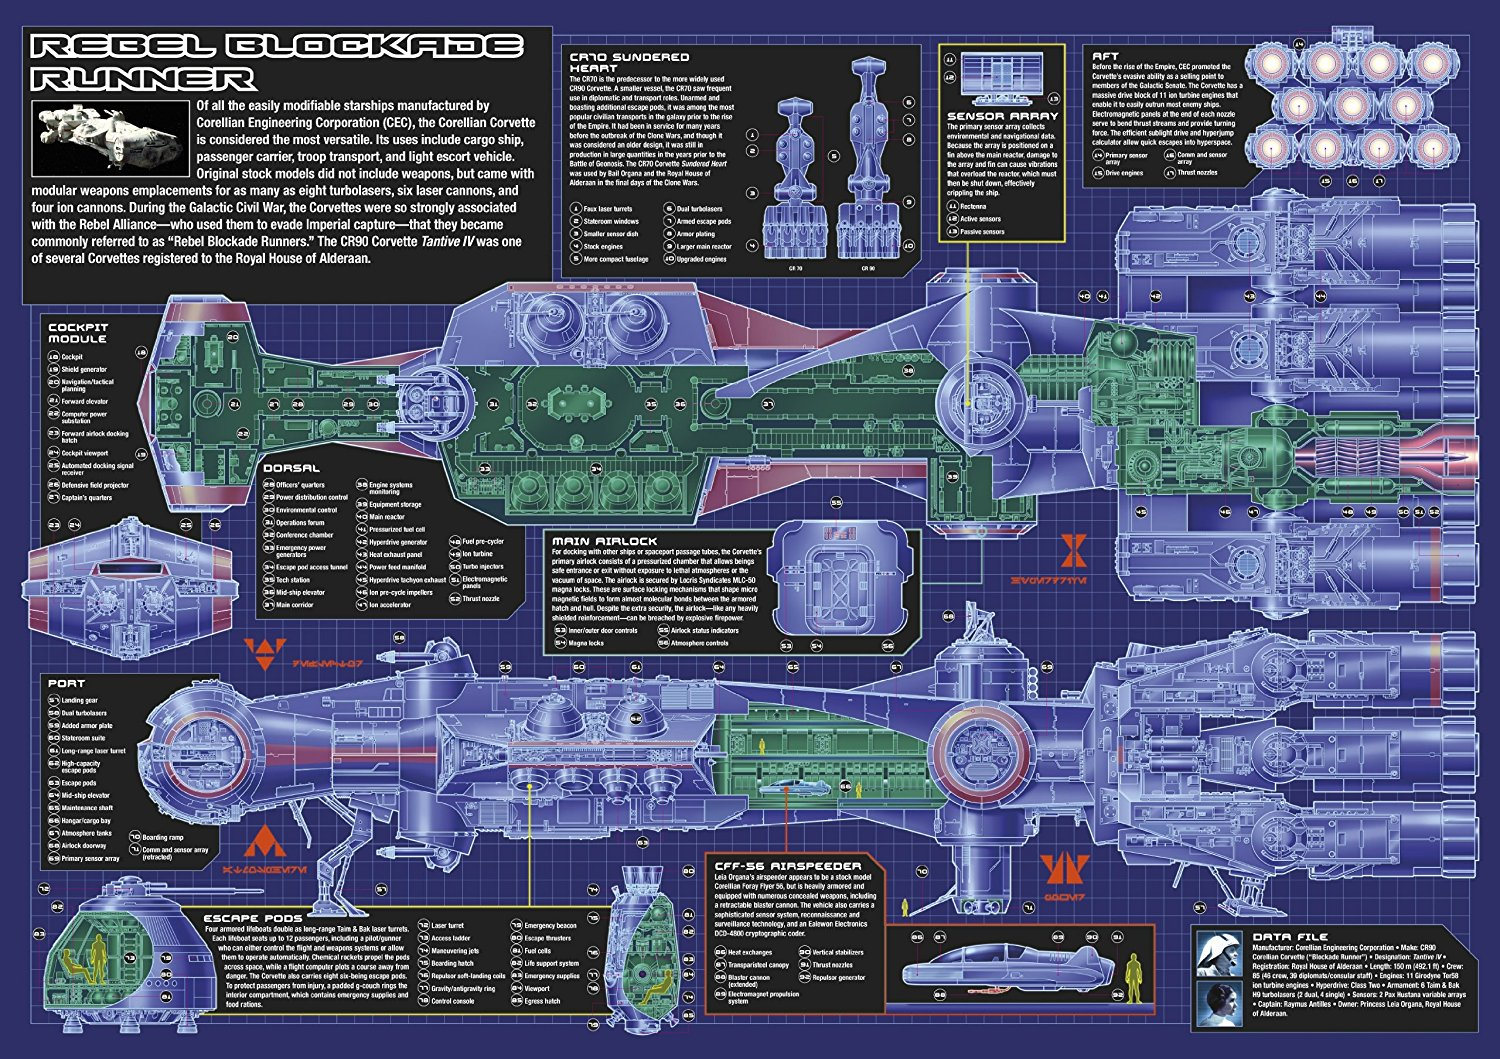
\includegraphics[width=1.0\textwidth]{img/vaisseau_echoue}
    \caption{Vaisseau échoué}
\end{figure*}

\chapter{Les pirates de l'espace}

\section{Une nouvelle mission}
\subtitle{22 octobre 2017}

Après quelques jours de repos et d'emplettes sur IsoOne, Nopok nous propose, par le biais de son organisme de chasseur de primes, de nous occuper quelque peu sur une nouvelle mission.

En effet, le consortium de Zan a quelques soucis avec un groupe de pirates et propose une belle récompense pour ceux qui peuvent lui régler ce problème.

Nous entrons donc en contact avec une pantorienne du nom de Venlana et d’une belle couleur bleue. Venlana se méfie des réseaux de communication et nous invite à la rejoindre sur Saleucami.

\begin{wrapfigure}{O}{0.5\columnwidth}
    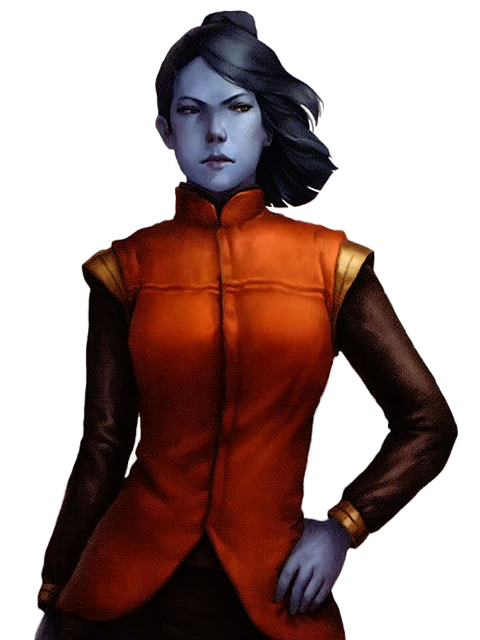
\includegraphics[width=0.5\columnwidth]{img/venlana.png}
    \caption{Venlana}
\end{wrapfigure}

Nous  partons donc d’IsoOne et laissons Reom et Cratala avec qui nous restons en bon termes (nous pourrons toujours les contacter à IsoOne).

Nous arrivons sur Saleucami, une planète très chaude en été … et nous sommes en été. La vie sur cette planète se passe plutôt de nuit vu la chaleur.

\begin{wrapfigure}{O}{0.25\textwidth}
    
\includegraphics[width=0.25\textwidth]{img/saleucami}
    \caption{Saleucami}
\end{wrapfigure}

Nous accostons sur le quai 75 et ne trouvons pas d’activités suspectes, malgré un très haut niveau de sécurité. Venlana nous attendait avec impatience car dès que nous sommes arrivés, elle nous contacte pour nous donner rendez-vous au \emph{Paradis}.

À la vue du niveau de sécurité, je me décharge (comme la plupart de mes compagnons) de mes armes illégales. Star Killer repère un passage pour les droïdes et choisi de sortir du hangar par cette sortie dérobée accompagné de notre droïde TI08. Ils arrivent à passer de justesse sans se faire remarquer car les gardes se sont plutôt occupés de caisses mal empilées qui sont tombées …

Nous nous retrouvons dehors et nous dirigeons vers le \emph{Paradis}. En chemin, nous sommes suivi par un gang local qui s’avère être les \emph{thaléos jaune}.

Au bar, Venlana nous attend et nous expose l’objectif du contrat. Ses activités sont régulièrement perturbées par les pirates de la sororité  voilée, dirigé exclusivement par un groupe de femmes. Elle nous propose 60\ 000 crédits pour la mission et nous indique quelques pistes pour les trouver:

Contacter Graf Lind qui a travaillé avec les pirates

Geo Wasento qui revend du matériel volé par la sororité

Hacker le serveur Sororinet, qui est une agence de voyage mais semble masquer quelque chose.
Star Killer, Karka et TI08 choisissent de rencontrer Graf Lind et nous, de notre côté, nous allons tenter de nous infiltrer dans la sororité en contactant Geo Wasento.

Geo est un rodien tenant un magasin sur Saleucami. Le magasin semble tout à fait légal. Ne voulant pas tourner autour du pot, nous abordons directement le sujet de la sororité. Geo n’est pas du tout à l’aise avec la discussion et finit par ordonner à son robot de nous attaquer et s’enfuit par l’arrière du magasin.

Dans la précipitation, je tente de le suivre sans succès dans l’arrière-boutique et Nopok fait directement le tour du magasin. Il arrivera à le rejoindre sans problème mais voulant les rattraper, je me perds dans les ruelles avoisinantes et me fait encercler par quelques vauriens.
Vite submergé par ces vauriens, je tente de discuter pour calmer le jeu. Heureusement, Nyr Ch'iort arrive à me retrouver. Embusquée légèrement plus loin, elle tente de s’attaquer au groupe. Malheureusement, elle rate complètement son attaque, mais c’est sans compter sur sa chance légendaire qu’elle arrive à détruire un panneau plus haut dans la ruelle qui s’abat sur mes adversaires. C’est ainsi qu’ils prennent la fuite et que nous retournons vers Nopok pour le questionner.

Les discussions nous mènent vers une certaine Mandy au cratère de “SombreVent”. Geo est vraiment inquiet de nous avoir donné ces informations et n’attend qu’une seule chose, prendre quelques vacances au vert. Pour la peine, nous récupérons les kits d’esclave cybernétique d’une valeur de 5000 crédits.

Nous rejoignons donc les autres au “Paradis” et les retrouvons quelque peu amochés aux côtés d’un ivrogne qui est en fait Graf Lind. Il nous confirme que Mandy est bien dans la sororité et qu’il connaît le cratère: il est à 200 kms d’ici.

Nous sommes encore un peu légers en Intel et Karka pirate donc le serveur de la sororité. Il y arrive plutôt facilement et recueille quelques informations indispensables pour arriver sur le site.

La sororité semble bien présente au cratère de \emph{SombreVent}, mais au sud du cratère. Le site est actif et attendent encore du matériel dans les deux jours. On estime que le site accueille une trentaine de personnel et qu’il est assez bien défendu, notamment par deux tourelles.

L’infiltration ne sera pas si simple.

\section{L’attaque du cratère}
\subtitle{26 novembre 2017}

Le jour pointe le bout de son nez et nous choisissons de nous reposer au \emph{Banta assis} afin de laisser passer les fortes chaleurs auxquels mes camarades ne sont pas habitués. Cette journée de repos nous permet de retrouver non seulement nos forces, mais aussi notre ami Wootang.

Nous préparons nos plans pour remplir le contrat. Afin d’être le plus discret possible, nous passons à EuroSpeeder pour louer un véhicule et nous nous dirigeons avec Graf vers le repère des pirates. Cette planète est bien étrange et nous y découvrons de nombreuses espèces différentes, comme des troupeaux de galvas sur la route ou encore des thaleos que nous ne ferons qu’entendre dans les bois. Il s’avère que les galvas peuvent être une bonne source de revenus à 100 crédits pour leur peau tannée.

Les parois du cratère sont assez escarpées et nous l’atteignons par l’ouest. Nous tentons d’en faire le tour par le Sud afin de trouver une entrée discrète, mais rien de bien praticable et discret. Nous arrivons tout de même à identifier la position de la base. Nous retournons donc sur nos pas pour pénétrer dans le cratère par l’Ouest.

Après avoir abandonné le speeder, nous progressons assez difficilement dans la jungle de nuit, car nous avons 6 kilomètres à parcourir. Cette faible distance nous offre quelques surprises.
Tout d’abord, nous nous faisons surprendre par un groupe de 5 clones assez âgés. Mais malgré leur âge, nous ils nous donnent pas mal de fil à tordre et nous amenuisent nos stimpacks et vide mon arme ! Ensuite, c’est la faune locale qui nous ralenti lorsque nous rencontrons un Nuuno (en genre de golem de pierre). Merci à Wootang et sa discrétion légendaire d’avoir réveillé la bête. StarKiller en arrive tout de même à bout.

Enfin, nous arrivons au repère des pirates. Avant d’attaquer la porte majestueuse et encadrée de meurtrières, nous nous reposons à l’ombre des pentes du cratère. La nuit venue, nous pénétrons dans le bâtiment tout en déclenchant les alarmes. Finalement, on nettoie le premier étage.

\subsubsection{Bilan !}

\begin{itemize}
    \item 18 morts dans le bâtiment
    \item 5 morts sur notre route
    \item Une arme vide
    \item Un sniper avec un bras en moins
    \item Beaucoup de stimpack en moins
    \item Pas mal de ratés en plus
\end{itemize}

\section{Et c'est pas fini !}
\subtitle{10 décembre 2017}

Maintenant, il faut que l’on attaque l’étage supérieur du repère !

Nous nous retrouvons au rez-de-chaussée, à la cuisine. Nous en profitons un peu pour nous reposer et nous alimenter grâce aux provisions que je trouve. Kar s’attaque à l’ordinateur et trouve qu’il devrait rester une quinzaine de personnes dans la base et surtout qu’une navette est en approche. Nous choisissons de continuer sur notre lancée et de continuer notre attaque.

Seule voie d’accès à l’étage: l’ascenseur … pour quatre. Star, Wootang, Nopok et Nyr montent donc à l’étage après que j’ai débloqué l’ascenseur. Mais dès que les portes s’ouvrent, un détonateur thermique leur arrive dessus. Star arrive à le dévier mais le souffle de l’explosion fait de nombreux dégâts. Nopok, déjà bien affaibli ne survit pas à ces ultimes blessures.

StarKiller arrive à décimer le groupe de 4 personnes dans la pièce en face qui s’avère être l’armurerie. Lorsque je m’apprête à prendre l’ascenseur, je constate le pauvre cadavre de Nopok et l’absence de Star. Nous remontons donc de suite pour tenter de lui prêter main forte. A la sortie de l'ascenseur, je tente un rapide coup d’œil pour repérer les autres ennemis mais je suis accueilli par une salve de tirs de blasters qui me mettent KO. Nyr me soigne vite fait pour continuer le combat.

Sous les feux nourris, nous tentons d’attaquer lourdement, mais même les grenades ne semblent toucher leur cible. Nous arrivons tout de même à avancer péniblement en nous barricadant à l’aide des caisses d’armes.

Ce maigre rempart nous permet de rejoindre StarKiller à l’armurerie, recharger mon arme et avancer dans le hangar adjacent. Star tente de lancer quelques grenades, mais malheureusement, le tir est mal ajusté et il en subit les dégâts.

Nous continuons l'assaut, il faut en venir à bout. Nyr part devant et je reste en retrait pour couvrir ses arrières. On voit les portes se fermer, ce doit être Kar qui a réussi à hacker le système informatique de la base. Sous nos tirs croisés, nous arrivons à nettoyer le hangar mais les dommages ont été lourds. Wootang nous requinque tous et choisissons de nous attaquer à ce qui semblerait être la salle de contrôle, nous y avons entendu du bruit.

On se met en embuscade proche des portes et à leur ouverture, nous attaquons aveuglément. C’est une femme qui va tomber sous les coups de StarKiller, et il s’avère que c’est Mandy qui apparemment, avait bien monté les échelons de la sororité. Elle nous indique tout de même que la reine pirate est  dans la pièce voisine.

Nous continuons alors notre progressions et accédons à l’objectif de notre mission: la reine. Elle semble de petite stature avec son masque, mais les 10 sbires à ses côtés renforcent son image de pouvoir. Nous continuons nos attaques pour tous les décimer.

Finalement, nous récupérons le masque, pour preuve. Au moment de le lui ôter, son apparence change du tout au tout. Star essaie le masque pour comprendre ce phénomène étrange et il s’avère que ce masque permet de prendre l’apparence de la reine, comme un genre d’hologramme.

Nous retournons donc à Saleucami rencontrer Venlana. Elle récupère le masque pour l’identifier afin de valider la mission. Nous devrions avoir nos crédits dans deux jours. Sur ce, nous nous séparons pour faire ce que l’on a à faire.

StarKiller va à l’hôpital local pour se soigner, car durant l’affrontement, nous avons subi de graves blessures, et quant à lui, il a perdu un bras qu'il remplace par un robotisé.

Wootang trouve au marché noir une robe Jedi pour mieux se protéger. Quant à moi, j’installe une cuve à bacta dans le vaisseau pour nous soigner. Kar y plonge directement pour se soigner (1 PV toutes les 2 heures et 1 jet de soins de critique chaque jour).

Au bout d’une journée, Venlana revient anxieuse et nous annonce que ce n’était pas la reine pirate. Les attaques continuent de plus belle, et sont maintenant signée “Les reines ne meurent pas si facilement.” Venlana en est exaspérée et nous demande de mettre fin à ses agissements et se propose de doubler la prime promise si nous pouvons nous occuper de cette “autre” reine. Elle ne nous donne pas trop d’autre choix, mais nous sommes tout de même bien amochés. Il faut que nous nous fassions une petite santé et que nous nous équipions afin de continuer sereinement notre traque.


\section{Des gains impressionnants !}
\subtitle{17 février 2018}

% Emprunt 8000 du vaisseau pour mon blaster
% Emprunt 8000 du vaisseau pour opération des yeux.

On doit aller Ord Mantell pour trouver la vraie reine. J'achète mon blaster customisé pour 9\ 600 crédits, dès que nous arrivons sur la planète. Finalement, mes multiples blessures sont graves, je dois me faire implanter des yeux cybernétiques afin de pouvoir recouvrer la vue, il me faut encore débourser plus de 7500 crédits.

On arrive au continent de Worlport et nous parquons au hangar 15. Ici, un toydarien du nom de Gender nous accueil. On a tout de suite un rendez-vous avec Ilo Vendin, car il nous faut des laisser-passer. Quant à moi, je récupère vite mon matériel et retourne au vaisseau.

Je reçois directement une lettre de Gender, avec un petit mot, nous demandant d'aller au plus vite au district des joyaux, pour y rencontrer Ilo. Nyr et Wootang y vont, mais personnellement, je reste au vaisseau. Ils vont donc rencontrer un des responsables des paris illégaux de la planète.

Ils arrivent à la demeure d’Ilo, qui est lourdement armée. En échange pour les informations qu'il peut nous fournir, il nous demande un petit service~: truquer un match de lutte, ou bien livrer un paquet.

Le combat étant notre dada, nous choisissons de faire en sorte que ce ne soit pas la favorite qui gagne le combat de lutte. Pour cela, nous ne tergiversons pas et nous inscrivons Wootang comme concurrent.
Ce dernier ce débrouille très bien sur les premiers combats mais la tenante du titre est tout de même sacrément coriace.
C'est sans compter sur l'aide de Starkiller et de son pouvoir de la force (pour déboîter les genoux) que nous réussissons à remplir la mission.
Par la même occasion, nous faisons chacun le plein de trésorerie grâce aux différents paris que nous mettons sur \emph{notre} champion.

C'est ce premier service que Wootang accepte.

C'est ici que nous rencontrons "Kalcir", avec qui nous allons vivre pas mal d'aventures finalement.

\section{L'attaque du \emph{Sang du Renégat}}
\subtitle{18 mars 2018}

\begin{figure*}[]
\centering
    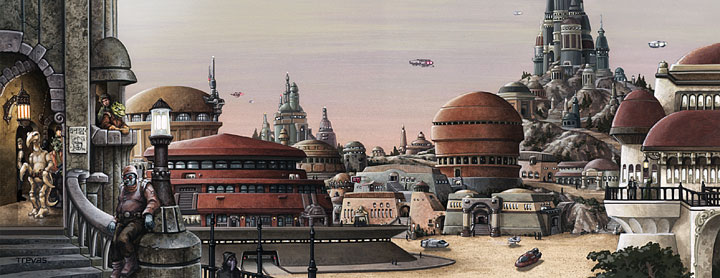
\includegraphics[width=.80\textwidth]{img/worlport}
    \caption{Cité de Worlport}
\end{figure*}

Encore à Worlport, on se prépare à décoller afin d'anticiper la prochaine attaque. Karka nous rejoint au vaisseau où nous lui présentons Kalcir Thuk.

De mon côté, j'ai récupéré JR12 afin de le réparer. En effet, les droïdes ont été lourdement endommagés lors de notre dernier combat. Nous avons même perdu notre astromech ! Je me dois de le renouveler. Avant de partir sur les coordonnées que nous avons récupérées, je répare JR12 et lui offre une partie des pièces de sa réparation. Nous restons ainsi amis, mais il ne souhaite pas nous accompagner dans nos aventures.

Nous décollons donc et voyageons rapidement vers les coordonnées que nous avons indiquées. Nous arrivons en pleine bataille spatiale ! Un vaisseau consulaire est devant nous, il se fait attaquer de toutes parts, mais en particulier, il est la cible de deux vaisseaux.

En observant la bataille, nous identifions notre cible, le \emph{Sang du Renégat}. On infiltre donc le vaisseau, pour atteindre la reine pirate, de la sororité voilée. Nous arrivons à elle, mais elle veut négocier dans un ultime espoir de survie. Ses arguments sont marquants ! Bien que pirate, elle lutte contre l'esclavage et l'injustice, que nous servons actuellement pour le compte du consortium de Zann. Nous choisissons alors de nous allier à elle.

Nous trahissons donc Venlana. Pour gagner du temps, nous faisons croire que nous sommes capturés, mais elle n'y croit pas du tout. Nous pouvons être sûrs à présent que quelques-uns vont penser à nous bien souvent !

\chapter{UPS - Universe Parcel Service}
\subtitle{2 septembre 2018 \newline Scénario custom}

Nous sommes donc à présent des pirates, au bandeau rouge\ : \emph{Aaaargh\ !}

La reine nous donne immédiatement 10\ 000 crédits, et nous promet les 10\ 000 autres en bonus de missions, puisque nous travaillons pour elle à présent.

Ord Mantell était la seconde base de la Sororité, celle-là même que j'ai infiltrée par le passé. Nous sommes donc de retour sur cette planète. Nyr est très proche de la reine, mais les autres pirates ne le sont pas du tout à notre encontre. Il faut avouer qu'on leur a fait pas mal de tort dans le passé.

Afin de clairement m'identifier au sein des pirates, je porte mon brassard rouge sur un de mes lekkus. Nous sommes assez tranquilles actuellement sur la planète, j'en profite pour retrouver mon ami JR12 ainsi que pour me soigner de mes différents maux. En discutant de ci, de là, nous apprenons que nos têtes sont mises à prix pour 2000 crédits. Ce n’est pas grand-chose ! Mais pour le groupe, ça commence à faire une somme rondelette.

% Achat d'un disrupteur pour 300 crédits

Au 3\ieme{} jour, nous sommes convoqués pour une nouvelle mission. C'est Sheina, une pantorienne plutôt coquine qui est accompagnée d'un slicer du nom de Vorak (gand) et d'un humain discret s'appelant Rook.

\begin{wrapfigure}{O}{0.5\columnwidth}
    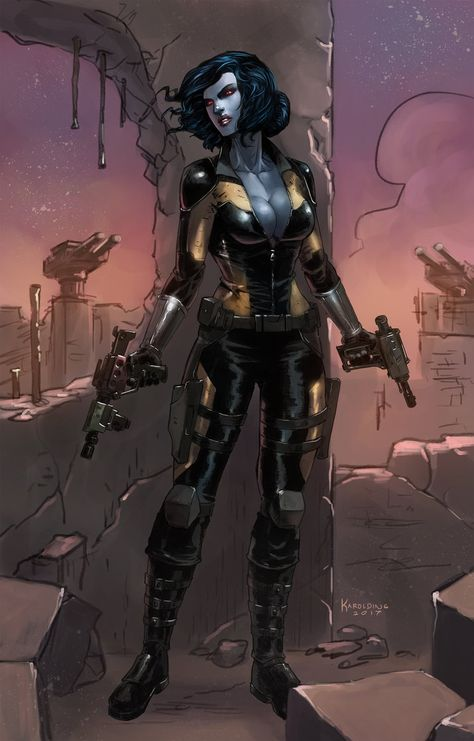
\includegraphics[width=0.5\columnwidth]{img/sheina}
    \caption{Sheina}
\end{wrapfigure}

La mission semble simple, ce qui tombe bien car quelques-uns de nos compagnons sont occupés. Seuls StarKiller, Wootang et moi sommes présents. La mission est de subtiliser quelque chose d'un entrepôt secret. Sheina reste très discrète sur l'objectif principal, mais le plan semble simple.

Se faire passer pour des livreurs, avec un chargement prévu, mais lors de la livraison, on repart mieux équipés ! Mais, c'est mal nous connaître\ !

Nous partons donc confiants vers Taleucemie. Nous livrons bien les caisses au laboratoire secret, caché sous le lac. Le plan se déroule sans accrocs\ ! Sheina récupère quelques fioles étranges et nous remontons à la surface. Ces fioles et le laboratoire sous-pressurisé me font penser plus à un virus qu'à autre chose. Mais je n'ai pas le temps de me poser plus de questions car lors de notre remontée, nous perdons contact avec Vorak, à bord du vaisseau.

Le vaisseau explose alors que nous nous en approchions\ ! Je me jette vers le hangar pour me protéger et mes autres compagnons se replient vers la base sous-marine. Sous les feux nourris, je me réfugie au fond du hangar afin de trouver une idée pour me sortir de ce guet-apens.

De leur côté, Sheina mène l'équipe au laboratoire sous-marin afin de repartir par le lac. Ils arrivent donc à sortir et longer la forêt afin de surprendre l'ennemi tapi dans les bois. Mais c'est sans compter sur la faune locale qui leur tombe dessus lourdement, dans la nuit noire et obscure.

Je reçois finalement quelques messages d'une voix inconnue qui, je l'espère est Rook. Il me signale que le terrain est dégagé, je prends donc le speeder du garage et le rejoins. Me voyant sous le coup de l'assaut, il prend les commandes du speeder et part à la recherche du reste de l'équipe.

Pendant ce temps, après s'être débarrassé des singes, ils ont pu localiser et attaquer nos assaillants. StarKiller a fait appel à la force pour les exterminer, et cela a suscité l'intérêt de Sheina, qui est de plus en plus \emph{intriguée} par lui.

Nos assaillants finissent par prendre la fuite. Nous reconnaissons finalement dans le groupe, Porel Vakra ! C'est le Twi’lek, garde du corps de Venlana. Elle nous en veut vraiment.


\cahpter{Il nous en manque un}
\subtitle{30 septembre 2018 \newline Scénario custom}

Nous retrouvons Nyr qui était en voyage avec la reine. Elle nous avoue que c'était sa tutrice, c'est pour cela qu'elle en est très proche. Kalcir quand a elle, finissait de régler ses affaires pour attaquer sa nouvelle vie avec nous. Quant à Karka, il travaillait dans son coin lors de notre dernière mission.

Nous sommes donc conviés auprès de la reine pour le debrief de la mission de livraison. Sheina lui donne la mystérieuse boite et nous sommes payés de 2000 crédits par personne, ce qui inclue la mission avec le bonus, promis pour rembourser les 10\ 000 en attente.

De mon côté, je répare complètement le vaisseau en 3 demi-journées.

\begin{quotebox}
En négociant avec JR12 pour obtenir une bonne adresse pour avoir un rabais de 20\%, j'arrive à réparer complètement le vaisseau.
\begin{itemize}
    \item 3 pts de coque pour 1200 crédits
    \item 6 pts de coque pour 2400 crédits
    \item 7 pts de coque pour 2800 crédits
\end{itemize}
\end{quotebox}

Kalcir nous apprend une bonne nouvelle ! Nous sommes encore plus recherchés ! Nos têtes sont passées à 3\ 000 crédits, morts ou vifs. Nous sommes tous recherchés, sauf elle. Et certains chasseurs de primes semblent être à nos trousses.

Les chasseurs de primes ne nous aiment pas, mais ce ne sont pas les seuls. Dans la base pirate, nous sentons que nous ne sommes pas les bienvenus. Certains nous en veulent pour notre assaut passé, d'autres nous prennent pour des assassins ou encore des profiteurs qui veulent prendre la tête de la Sororité.

Durant le repas, nous constatons l'absence de Nyr, Karka nous annonce qu'elle est partie seule à la banque !!! Impossible de la retrouver sur la base, même la reine n'a aucune nouvelles.
% Je récupère le numéro de comlink de la reine.
Nous partons donc à la recherche de notre coéquipière qui était partie en direction de la CIB. C'est Karka qui nous guide puisqu'il arrive à localiser le comlink.

Chemin faisant, StarKiller collecte quelques informations \emph{gentiment} et nous arrivons à une planque avec un guetteur. Sans hésiter, Kalcir a la gâchette facile et le descend froidement. Nous investissons les lieux, il faut retrouver notre pilote !

Karka est contacté directement par les ravisseurs et menacent de tuer Nyr !

Pas question de renoncer\ ! Malgré le coup de feu, on fouille l'immeuble et même les bâtiments voisins\ ! Du sol au toit ! Ils nous ont vus arriver, c'est qu'ils ne doivent pas être loin.

Finalement, nous la retrouvons dans la ruelle, amochée et sans équipement. Nous remontons la trace de son échappée grâce à ses bribes de souvenirs. En effet, nous n'avions pas fouillé les caves. C'est là qu'ils se sont planqués.

On retrouve ses affaires, mais aucune trace de ses ravisseurs. Nous rentrons donc à la base pour nous remettre de toutes ces émotions.

\chapter{Joyau de Yavin}

Après une bonne nuit réparatrice, nous partons pour une mission confiée par la reine. Ça permettra de faire profil bas sur la planète, car d'un côté les pirates ne nous apprécient pas et de l'autre, nos têtes sont bien misent à prix. La mission n'est pas très claire, c'est sur Bespin que notre contact nous donnera de plus amples informations.

\begin{wrapfigure}{O}{0.5\columnwidth}
    
\includegraphics[width=0.5\columnwidth]{img/bespin_poster}
    \caption{Bespin}
\end{wrapfigure}

% 40 crédits d'atterrissage et on se pose sur le parvis.

En arrivant à la cité des nuages, nous appelons notre contact qui nous donne rendez-vous au Souk, à un marchand de tissus. C'est donc dans un immense dédale d'échoppes que nous devons la retrouver. En chemin, nous nous renseignons plus sur cette planète et apprenons qu'un certain Lobot gère toute l'informatique sur cette planète. Si jamais, nous sommes amenés à toucher au réseau, on aura affaire à lui. Non seulement en informatique, ils sont plutôt \emph{high level} ici, mais leur garde ailée est tout aussi redoutable et zélée. C'est finalement un peu comme la roue que nous avons fréquentée dans le passé. 

Nous laissons Kalcir contacter notre indicateur, puisque c'est la moins connue du groupe. C'est une pantorienne qui vient à nous. Mais elle est suivie par toute une bande de gars vêtus de noir, menés par un luthréen. On arrive à divertir toute cette équipe en mettant la pagaille dans le souk, au prix de quelques fruits et chandeliers\ \emph{?!?!} reconvertis en armes improvisées. Finalement, ces gars n'en avaient pas après nous, mais après cette pantorienne.

Elle nous file une clef d'appartement afin qu'on puisse discuter plus calmement de la mission.

Au nouveau lieu de rendez-vous, nous faisons connaissance d’Aris et de son père Arend Shen. C'est lui qui nous présente la mission pour laquelle nous sommes engagés.

Dans quelques jours, le joyau de Yavin va être mis en vente et il nous demande de rafler le tout. C'est à dire\ : faire monter les enchères, voler l'argent du transfert \textbf{ET} voler la pierre.

Cette pierre appartient pour l'instant à Marcus Grayson, c'est un brigand très puissant, et l'un des enchérisseurs est le propre mari d’Aris. C'est lui qui a fait suivre son épouse et elle n'est pas contre que nous lui fassions un mauvais tour. Drôle de famille.

Harren propose de nous soutenir si besoin dans cette mission, afin de monter le casse le plus efficacement possible. Il nous conseille de nous intéresser à la grande course qui va avoir lieu prochainement, car l'équipe gagnante pourra assister à la vente, il ne propose même un véhicule. Mais ceci ne répondrait qu'à un seul des objectifs\ ! Car il faudra faire monter les enchères, malgré que la liste des acheteurs soit close, ensuite il faudra détourner l'argent du transfert alors qu'il sera assuré par un droïde financier et pour finir, on devra repartie avec le joyau de Yavin.


\section{Ocean 6}
\subtitle{20 janvier 2019}

\begin{figure*}[]
\centering
    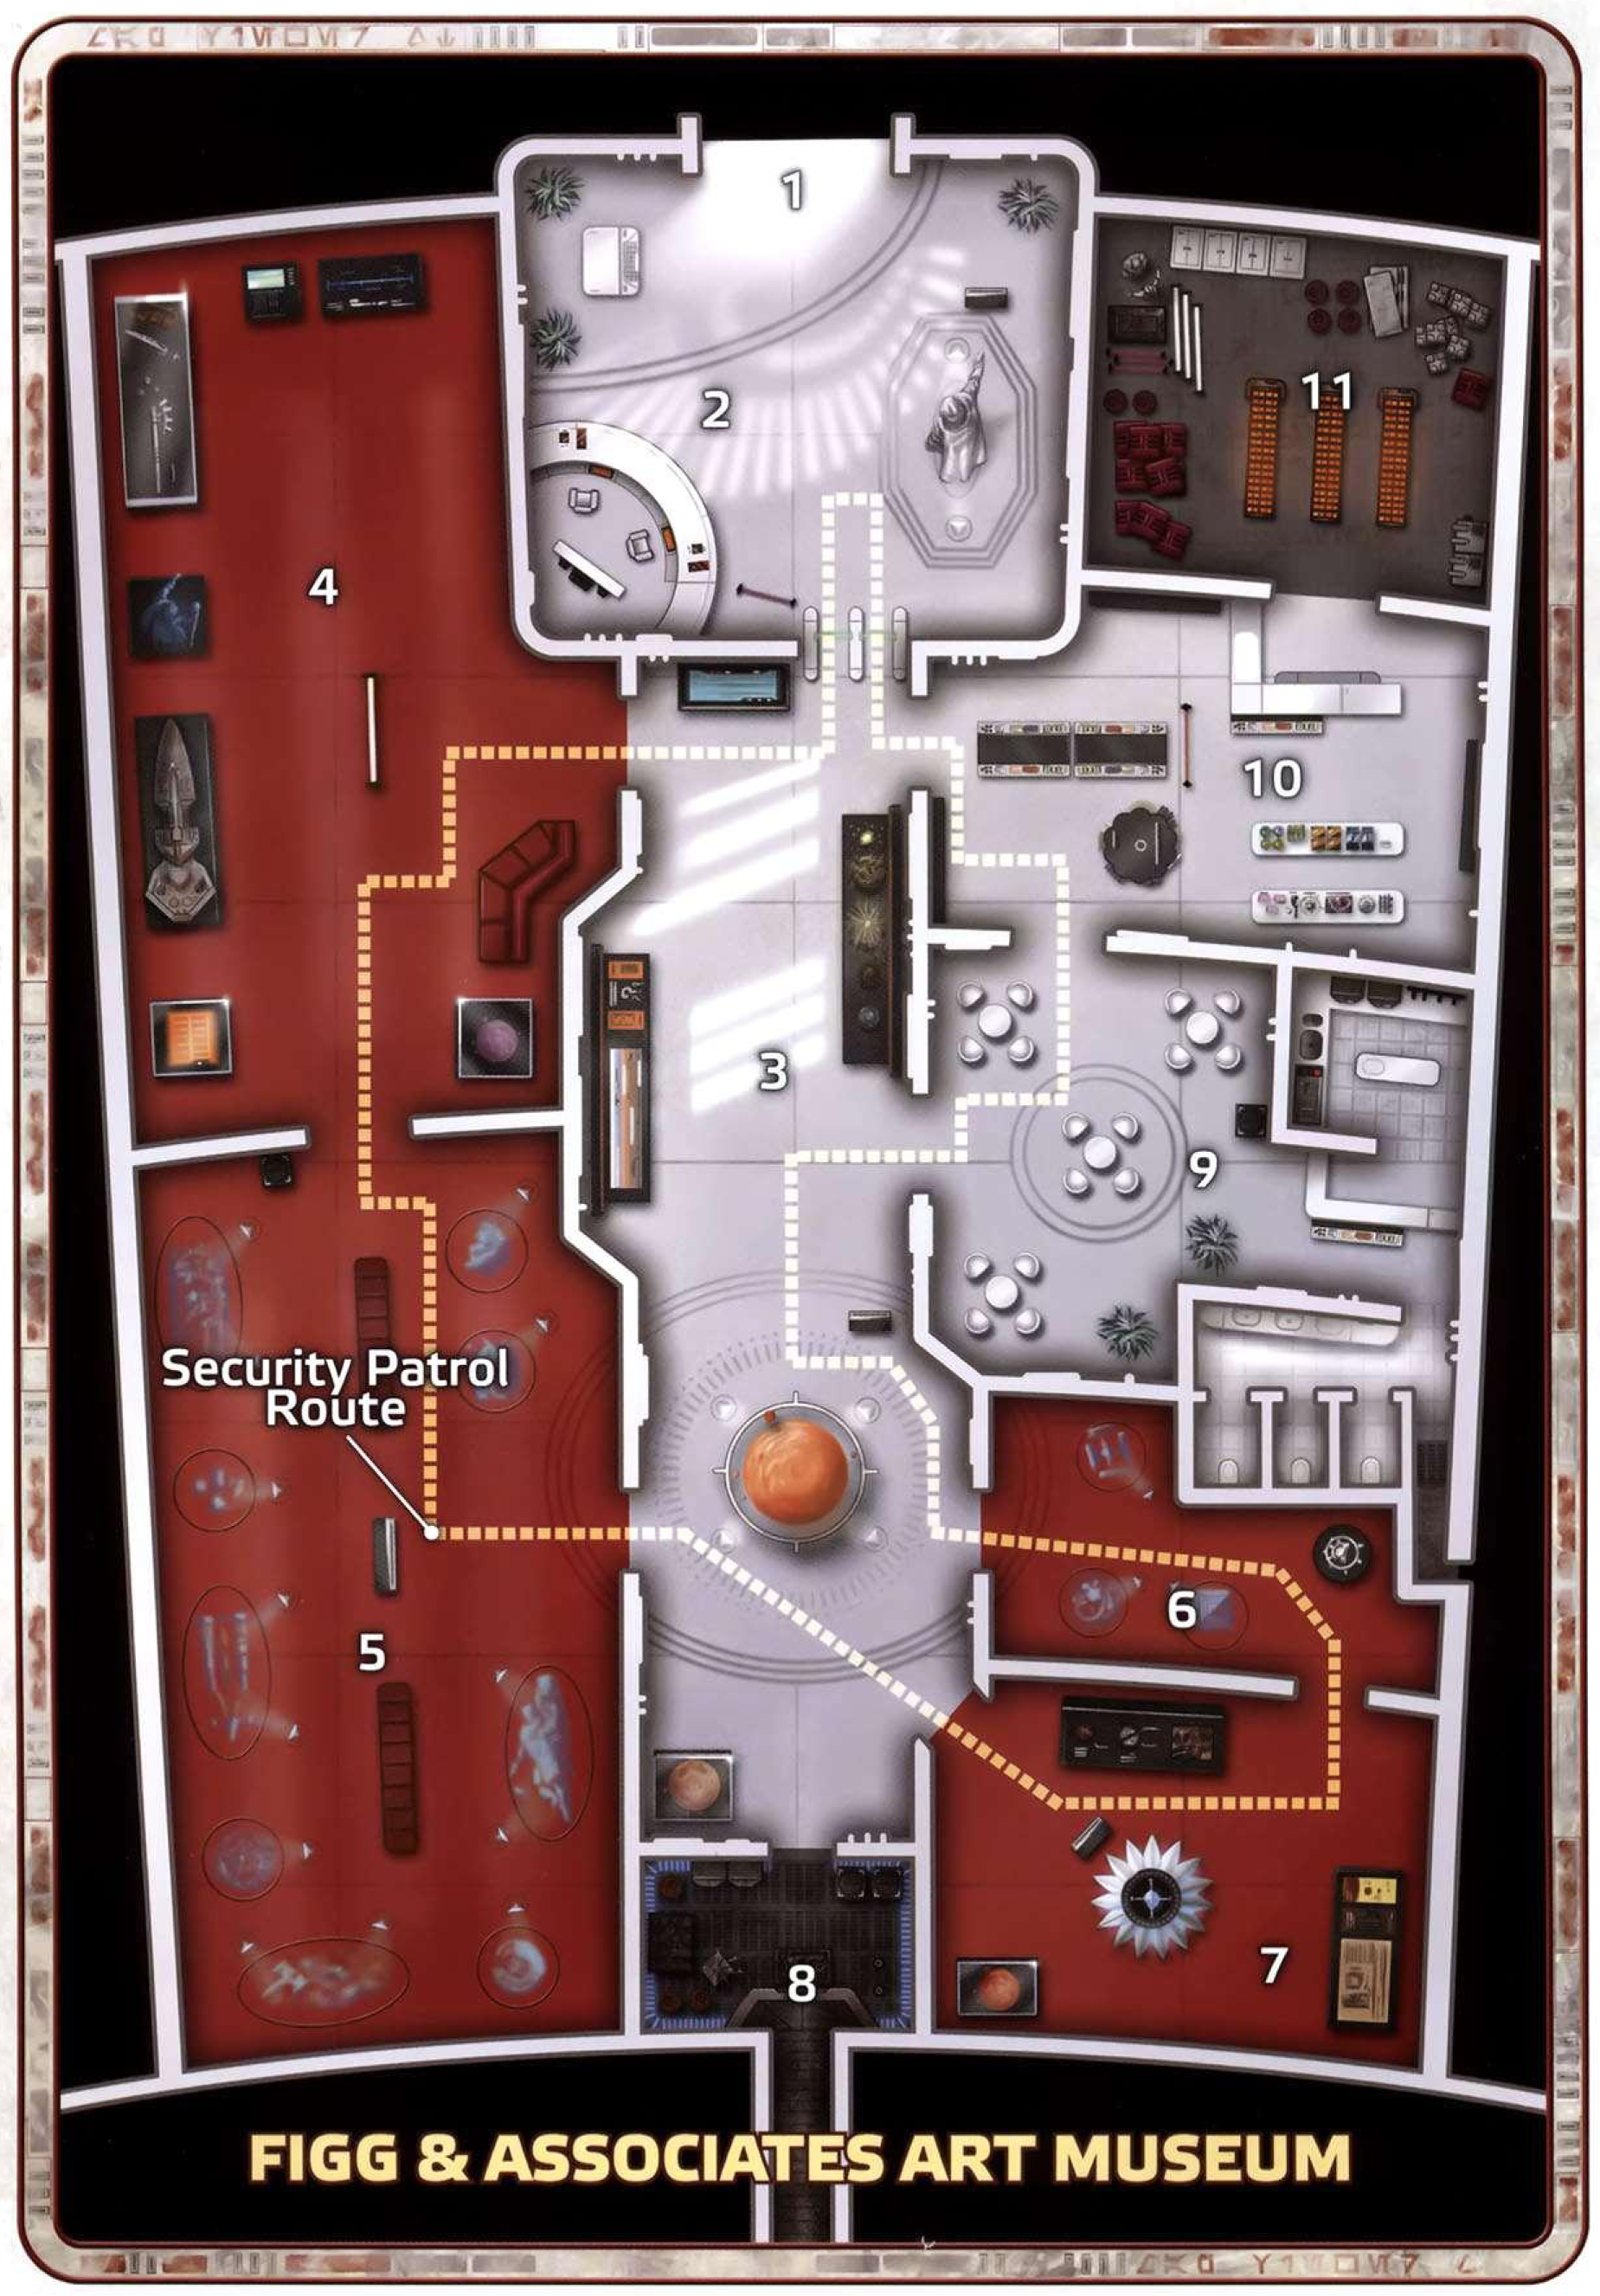
\includegraphics[width=.80\textwidth]{img/YavinMuseum.png}
    \caption{Musée de Bespin}
\end{figure*}

Afin de se préparer à la mission, nous prenons place à l'hôtel modeste de \emph{Dame Adiarite}. Cette auberge est tenue par \emph{Bozzi}, une Ughnaute. J'en profite pour lui parler de certaines connaissances communes dans sa communauté afin d'obtenir quelques contacts de confiance. C'est ainsi, qu'elle m'orientera vars \emph{Negri}.

Pendant que la plupart du groupe se retrouve à la cantina \emph{La retraite}, je vais vers le dock privé où je pourrai préparer le bolide pour la course. J'y trouve un pod de la garde ailée qu'il faut finir de préparer.

\begin{figure*}[]
\centering
    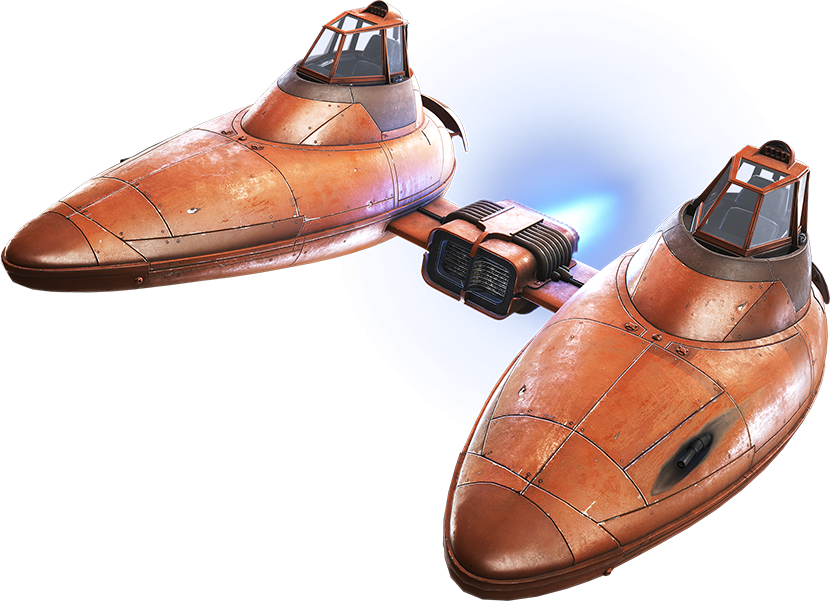
\includegraphics[width=.80\textwidth]{img/cloud-car-v2.png}
    \caption{Voiture des nuages}
\end{figure*}

Ce véhicule est très performat, mais je passe tout de même toute la nuit pour l'améliorer afin de pouvoir le pousser dans le moindre de ses retranchements. Ainsi, je lui apporte plusieurs modifications:

\begin{itemize}
\item Propulseur secondaire
\item Turborépulseur
\item Amplificateur de mémoire
\end{itemize}

Toutes ces modifications me coûte 3000 crédits grâce à notre contact Negri qui tient une turbine. C'est par cet individu que nous pourrons nous débarrasser de \emph{trucs} embêtant ou bien sortir discrètement des objets que nous pouvons dissimuler dans de la carbonite.

Le joyau de \emph{Yavin} est donc notre cible. J'ai appris que cette pierre date de la grande guerre des Siths. C'est une pierre dite maudite surnommée \emph{Incassable} car personne n'a jamais pu la voler. Nous nous faisons foi de prouver le contraire.

Pendant ce temps là, mes comparses s'attellent à différentes tâches afin de préparer au mieux le casse impossible. Notre slicer s'occupe de préparer le hack pour détourner l'argent, tout en évitant \emph{Lobos}. On réunit donc tout ce dont nous avons besoin :
\begin{itemize}
\item Pistolet ionique
\item Brouilleur (400 crédits)
\item Bouchon d'entrave
\item Clef de reprogrammation
\end{itemize}

Ainsi, nous préparons notre plan d'action:
\begin{enumerate}
\item Préparer une diversion (explosion d'un stabilisateur de la ville) pour détourner Lobos
\item Fin de l'enchère
\item Vol du diamant
\item Hack du robot
\item Destruction du robot (par le biais de Negri)
\item Départ vers de nouvelles aventures
\end{enumerate}

Le grand jour arrive donc, afin de mettre notre plan à exécution.

\section{D-Day}
\subtitle{17 février 2019}

Le grand jour de la course et du casse arrive ! L'équipe de la course déjeune ensemble et nous tentons de lier connaissance avec Elesa qui est l'une des enchérisseuse. Je n'arrive pas à recueillir des informations et elle part à ses affaires.

De mon côté, je prépare une bombe électromagnétique pour le stabilisateur de la ville. J'ai repérer où la déposer et charge Wootang d'escalader le puits central pour déposer la bombe. En chemin, il rencontre quelques ordures mais aussi des animaux qui hantent ce vide ordure. Malgré ces péripéties, le \emph{colis} et déposé. Nous profitons de la course pour diminuer les risques de se faire surprendre.

Pendant ce temps, la course est menée de rondement par Nhyr, notre pilote. Durant toute la course, et grâce à la préparation du pod, elle garde un avantage certain sur ses adversaires. Cette course a été remplie de surprises ! Non seulement les concurrents peuvent être menaçants, mais la nature elle-même est un obstacle. Nhyr doit se sortir de la meute des concurrents tout en évitant les créatures sortant des nuages.

Bien qu'épaulée d'un artilleur hors-pair, ses qualités de pilote lui permettent de gagner la course haut la main.

Elle vient donc de gagner notre ticket d'entrée pour le gala.

Nous y allons donc tous ensemble pour tenter de faire monter les enchères. Exceptionnellement pour la soirée, je m'habille avec une nouvelle tenue de gala.

\begin{wrapfigure}{O}{0.5\columnwidth}
    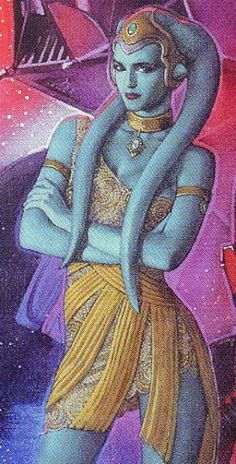
\includegraphics[width=0.5\columnwidth]{img/twilek_dress.jpg}
    \caption{Robe de Gala}
\end{wrapfigure}

Afin de monter les enchères, je discute, papote avec les différents intervenants. J'aborde aussi Elesa, mais elle disparaît assez vite de la salle de Gala. Je séduis un peu un autre enchérisseur et je pense avoir réussi ma mission.

\À la fin des enchères, je pars avec Karka pour détourner le virement. Durant l'après-midi, il a ouvert un compte en banque avec une fausse identité parfaite (pour 50 000 crédits, ça doit être en béton). Nous attaquons donc le droïde bancaire au moment ou je fais péter le stabilisateur afin de détourner l'attention de Lobos. Malheureusement, nous nous attaquons trop vite au droïde et il soupçonne tout de même notre hack. Karka arrive tout de même à le contrer et modifier le destinataire du virement.

Ensuite, nous nous débarrassons du droïde chez Negri. Après toutes ces aventures, je retourne au vaisseau pour préparer notre départ. Lors de mon arrivée, je constate que le hangar est bien gardé par des hommes de mains. Il me semble reconnaître ceux que l'on a rencontrés dès notre arrivée. Je parviens tout de même à pénétrer discrètement dans le hangar et rejoindre le vaisseau. Ils ont vraiment peur que nous leur fassions une entourloupe, car ils ont saboté le propulseur. Il me faudra bien une haure pour tout réparer.

Pendant ce temps là, Karka hack le système vidéo du musée pour que Wootang et Starkiller volent le joyau de Yavin.
Ce vol ne se fait pas sans peine, c'est un vrai carnage.
Ils éliminent tous les gardes. Starkiller s'avère maîtriser la force !
Tout comme Elesa qui leur demande le joyau. En effet, elle est présente au musée, dès la fin du cambriolage.

Starkiller semble vouloir lui donner ... Mais sous la menace de notre amie la loutre géante, elle s'enfuit. De même, Harren s'en vient aux nouvelles régulièrement pour savoir quand récupérer le joyau, mais mes acolytes ne semblent pas prêts à honorer le contrat ! Il semblerait bien qu'il se doute du manque d'intégrité de certains. Les hommes encerclant notre vaisseau sont sûrement des hommes à lui.

De mon côté, pendant que je répare le réacteur, les hommes de main sont entrés dans le hangar et me mettent en joue ...

\clearevenpage

% Création de la quatrième de couverture
\onecolumn
\Large

\centering

\vfill

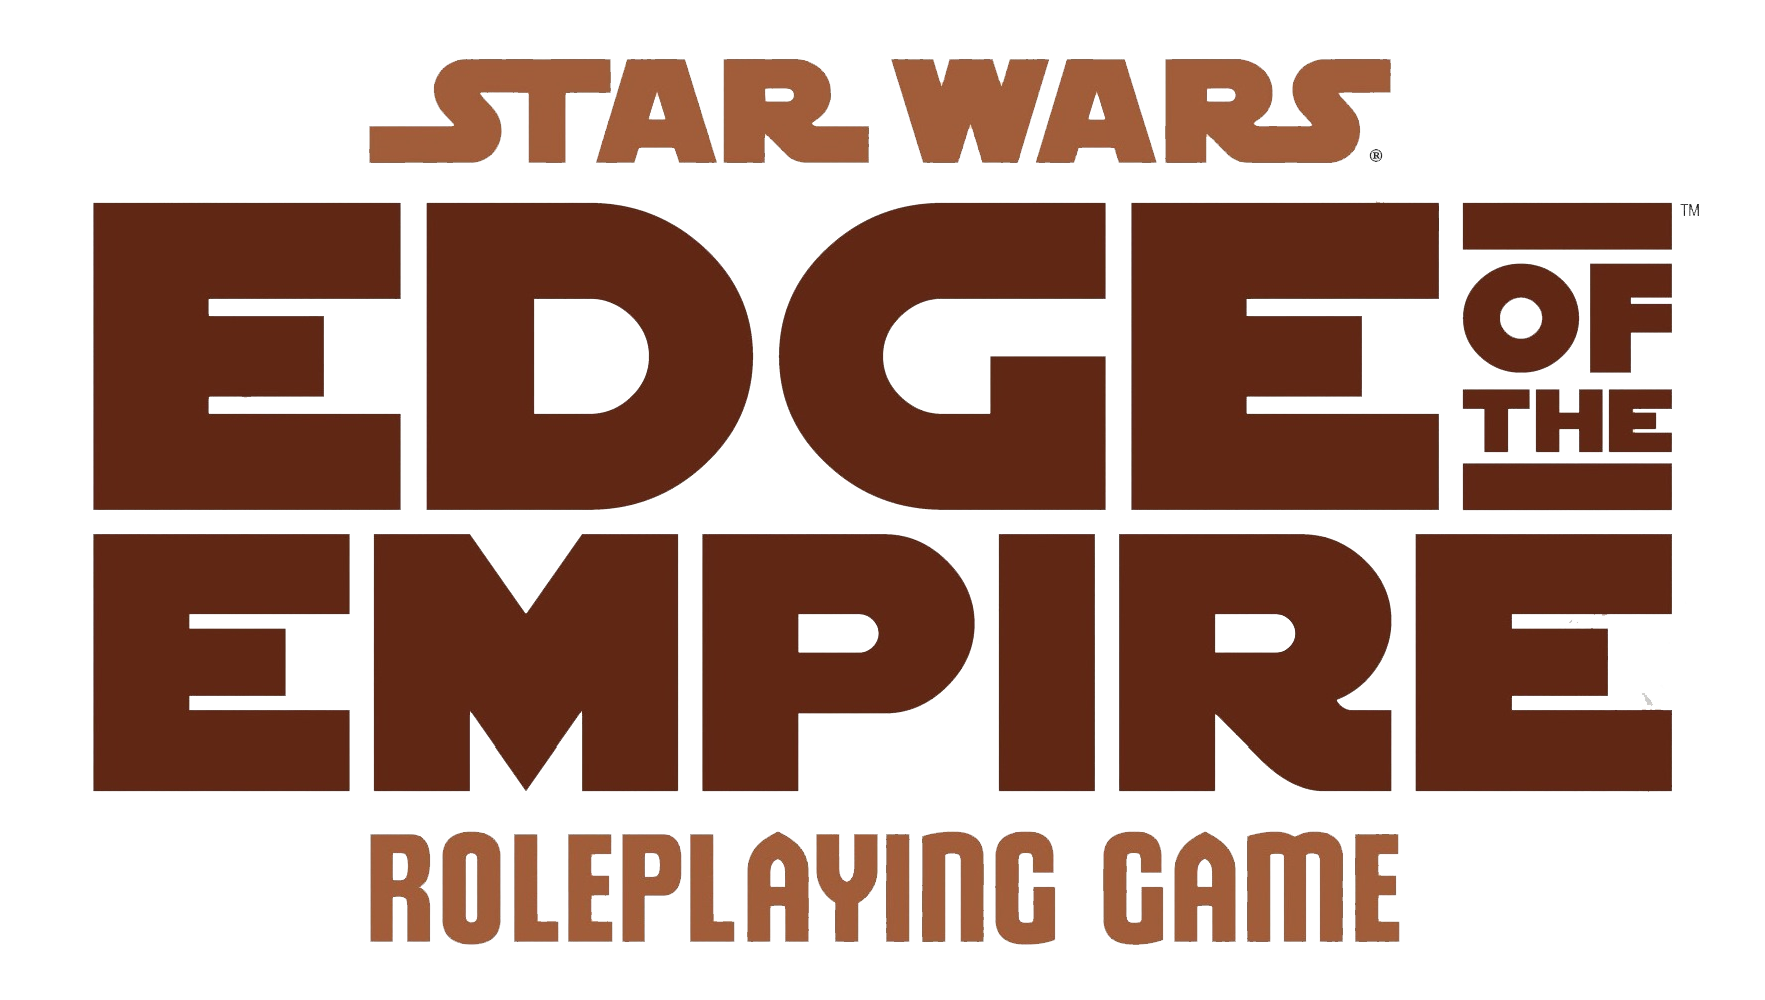
\includegraphics[width=1\textwidth]{img/SWEotE}


\vfill

L'histoire de quelques gars et demoiselles à travers l'espace.
\vfill

% End document
\end{document}
